% Paquets généraux
\documentclass[a4paper,12pt,titlepage]{article}
\usepackage[T1]{fontenc}
\usepackage[utf8]{inputenc}
\usepackage[french]{babel}
\usepackage[gen]{eurosym}
%\usepackage[dvips]{graphicx}
\usepackage{fancyhdr}
\usepackage{pdfpages} 
\usepackage{multido}
\usepackage{hyperref}
%\usepackage{textcomp}
%\usepackage{aeguill}
\usepackage{schemabloc}
\usepackage[bitstream-charter]{mathdesign}
\usepackage{minted}

\newcommand{\id}{71}
\newcommand{\nom}{Théorie des mécanismes}
\newcommand{\sequence}{04}
\newcommand{\nomsequence}{Liaisons entre les solides}
\newcommand{\num}{02}
\newcommand{\type}{KH}
\newcommand{\descrip}{Liaisons équivalentes, hyperstatisme, liaisons en série et en parallèle, théorie des graphes}
\newcommand{\competences}{B2-12: Proposer une modélisation des liaisons avec leurs caractéristiques géométriques. \\ &  B2-13: Proposer un modèle cinématique paramétré à partir d'un système réel, d'une maquette numérique ou d'u \\ &  B2-17: Simplifier un modèle de mécanisme. \\ &  B2-18: Modifier un modèle pour le rendre isostatique. \\ &  C1-04: Proposer une démarche permettant d'obtenir une loi entrée-sortie géométrique.  \\ &  C2-05: Caractériser le mouvement d'un repère par rapport à un autre repère. \\ &  C2-06: Déterminer les relations entre les grandeurs géométriques ou cinématiques. }
\newcommand{\nbcomp}{7}
\newcommand{\systemes}{}
\newcommand{\systemesnum}{}
\newcommand{\systemessansaccent}{}
\newcommand{\ilot}{2}
\newcommand{\ilotstr}{02}
\newcommand{\dossierilot}{\detokenize{Ilot_02 }}


\newcommand{\auteurun}{Renaud Costadoat}
\newcommand{\auteurdeux}{Françoise Puig}
\newcommand{\institute}{Lycée Dorian}


\usepackage{color}
\usepackage{xcolor}
\usepackage{colortbl}
\usepackage{helvet}
\usepackage[frenchmath]{newtxsf} % for sans serif symbols
\renewcommand{\familydefault}{\sfdefault}
%\usepackage{amsfonts}
%\usepackage{amsmath}
%\usepackage{lmodern}
\usepackage{mathastext}
%\usepackage{xspace}
\usepackage{varioref}
\usepackage{tabularx}
%\usepackage{floatflt}
\usepackage{graphics}
\usepackage{wrapfig}
\usepackage{textcomp}
\usepackage{tikz}
\usepackage{wrapfig}
\usepackage{gensymb}
\usepackage[european]{circuitikz}
\usetikzlibrary{babel}
\usepackage{ifthen}
\usepackage{cancel}
\usepackage{etoolbox}
\usepackage{multirow}
%\usepackage{boxedminipage}
\definecolor{gris25}{gray}{0.75}
\definecolor{bleu}{RGB}{18,33,98}
\definecolor{bleuf}{RGB}{42,94,171}
\definecolor{bleuc}{RGB}{231,239,247}
\definecolor{rougef}{RGB}{185,18,27}
\definecolor{rougec}{RGB}{255,188,204}%255,230,231
\definecolor{vertf}{RGB}{103,126,82}
\definecolor{vertc}{RGB}{220,255,191}
\definecolor{forestgreen}{rgb}{0.13,0.54,0.13}
\definecolor{blcr}{rgb}{0.59,0.69,0.84}
\definecolor{blfr}{rgb}{0.32,0.51,0.75}
\definecolor{orfr}{rgb}{0.90,0.42,0.15}
\definecolor{orcr}{rgb}{0.90,0.65,0.50}
\definecolor{orangef}{rgb}{0.659,0.269,0.072}
\definecolor{orange}{rgb}{0.58,0.35,0.063}
\definecolor{orangec}{rgb}{0.43,0.32,0.25}
\definecolor{rcorrect}{rgb}{0.6,0,0}
\definecolor{sequence}{rgb}{0.75,0.75,0.75}
\definecolor{competences}{rgb}{0.61,0.73,0.35}
\definecolor{grisf}{HTML}{222222}
\definecolor{grisc}{HTML}{636363}
\definecolor{normal}{HTML}{4087c4}
\definecolor{info}{HTML}{5bc0de}
\definecolor{success}{RGB}{92,184,92}
\definecolor{warning}{RGB}{240,173,78}
\definecolor{danger}{RGB}{217,83,79}
\hypersetup{                    % parametrage des hyperliens
    colorlinks=true,                % colorise les liens
    breaklinks=true,                % permet les retours à la ligne pour les liens trop longs
    urlcolor= blfr,                 % couleur des hyperliens
    linkcolor= orange,                % couleur des liens internes aux documents (index, figures, tableaux, equations,...)
    citecolor= forestgreen                % couleur des liens vers les references bibliographiques
    }

% Mise en page
\pagestyle{fancy}

\setlength{\hoffset}{-18pt}

\setlength{\oddsidemargin}{0pt} 	% Marge gauche sur pages impaires
\setlength{\evensidemargin}{0pt} 	% Marge gauche sur pages paires
\setlength{\marginparwidth}{00pt} 	% Largeur de note dans la marge
\setlength{\headwidth}{481pt} 	 	% Largeur de la zone de tête (17cm)
\setlength{\textwidth}{481pt} 	 	% Largeur de la zone de texte (17cm)
\setlength{\voffset}{-18pt} 		% Bon pour DOS
\setlength{\marginparsep}{7pt}	 	% Séparation de la marge
\setlength{\topmargin}{-30pt} 		% Pas de marge en haut
\setlength{\headheight}{35pt} 		% Haut de page
\setlength{\headsep}{20pt} 		% Entre le haut de page et le texte
\setlength{\footskip}{30pt} 		% Bas de page + séparation
\setlength{\textheight}{700pt} 		% Hauteur de l'icone zone de texte (25cm)
\setlength\fboxrule{1 pt}
\renewcommand{\baselinestretch}{1}
\setcounter{tocdepth}{1}
\newcommand{\cadre}[2]
{\fbox{
  \begin{minipage}{#1\linewidth}
   \begin{center}
    #2\\
   \end{center}
  \end{minipage}
 }
}

\newcounter{num_quest} \setcounter{num_quest}{0}
\newcounter{num_rep} \setcounter{num_rep}{0}
\newcounter{num_cor} \setcounter{num_cor}{0}

\newcommand{\question}[1]{\refstepcounter{num_quest}\par
~\ \\ \parbox[t][][t]{0.15\linewidth}{\textbf{Question \arabic{num_quest}}}\parbox[t][][t]{0.93\linewidth}{#1}\par
}


\newcommand{\reponse}[1]
{\refstepcounter{num_rep}
\noindent
\rule{\linewidth}{.5pt}
\textbf{Question \arabic{num_rep}:}
\multido{\i=1+1}{#1}{~\ \\}
}

\newcommand{\cor}
{\refstepcounter{num_cor}
\noindent
\rule{\linewidth}{.5pt}
\textbf{Question \arabic{num_cor}:} \\
}

\newcommand{\titre}[1]
{\begin{center}
\cadre{0.8}{\huge #1} 
\end{center}
}


% En tête et pied de page
\fancypagestyle{normal}{%
  \fancyhf{}
\lhead{\nom}
\rhead{
\includegraphics[width=2cm]{../../img/logo}\hspace{2pt}}
\ifdef{\auteurdeux}{\lfoot{\auteurun,\auteurdeux}}{\lfoot{\auteurun}}
\cfoot{Page \thepage}}

\fancypagestyle{correction}{%
  \fancyhf{}
  \lhead{\colorbox{danger}{\begin{minipage}{0.65\paperwidth} \textcolor{white}{\textbf{Correction}} \end{minipage}} }
  \rhead{
\includegraphics[width=2cm]{../../img/logo}}
  \ifdef{\auteurdeux}{\lfoot{\auteurun,\auteurdeux}}{\lfoot{\auteurun}}
  \rfoot{\colorbox{danger}{\begin{minipage}{0.5\paperwidth} \begin{flushright}\textcolor{white}{\textbf{Correction}}\end{flushright} \end{minipage}} }}

\renewcommand{\footrulewidth}{0.4pt}

\usepackage{eso-pic}
\newcommand{\BackgroundPic}{%
\put(0,0){%
\parbox[b][\paperheight]{\paperwidth}{%
\vfill
\begin{center}
\hspace{0.5cm}\vspace{0.5cm}

\includegraphics[width=\paperwidth,height=\paperheight,%
keepaspectratio]{../../img/fond3}%
\end{center}
\vfill
}}}

\newcommand{\BackgroundPicdeux}{%
\put(25,-30){%
\parbox[b][\paperheight]{\paperwidth}{%
\vfill
\begin{center}
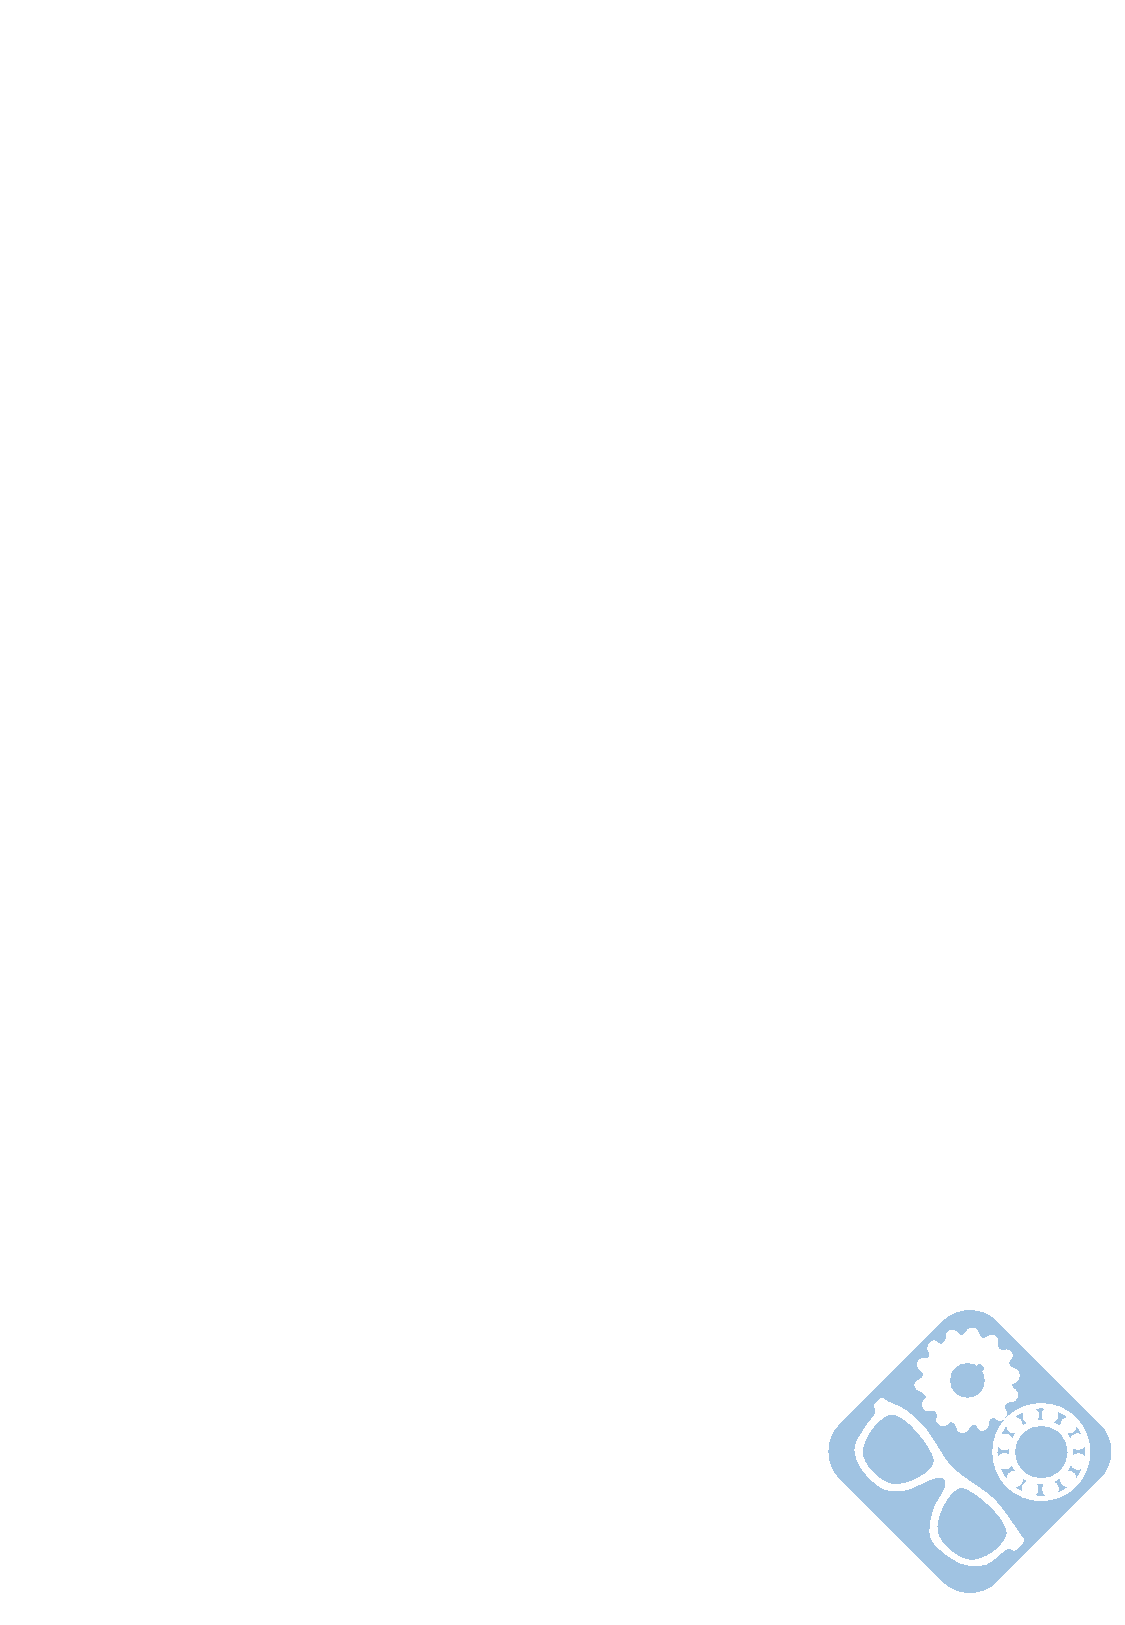
\includegraphics[width=\paperwidth,height=\paperheight,%
keepaspectratio]{../../img/fond4}%
\end{center}
\vfill
}}}

\begin{document}

\pagestyle{empty}

\vspace*{-3\baselineskip}

\AddToShipoutPicture*{\BackgroundPic}

\ifdef{\auteurdeux}{\begin{tabular}{>{\columncolor{gray!00}}m{.3\linewidth} m{.3\linewidth} >{\columncolor{gray!00}}m{.3\linewidth}}
Séquence : \sequence &  \multirow{3}{*}{\hspace{1cm}
\includegraphics[height=1.5cm]{../../img/logo}} &  \begin{flushright} \multirow{4}{*}{\hspace{1cm}\includegraphics[height=4cm]{img/qrcode}}\end{flushright}\\
Document : \type\num \\
 \institute \\
 \auteurun\\
 \auteurdeux
\end{tabular}}{\begin{tabular}{>{\columncolor{gray!00}}m{.3\linewidth} m{.3\linewidth} >{\columncolor{gray!00}}m{.3\linewidth}}
Séquence : \sequence &  \multirow{3}{*}{\hspace{1cm}
\includegraphics[height=1.5cm]{../../img/logo}} &  \begin{flushright} \multirow{4}{*}{\hspace{1cm}\includegraphics[height=4cm]{img/qrcode}}\end{flushright}\\
Document : \type\num \\
 \institute \\
 \auteurun
\end{tabular}}

\vspace{1cm}

\ifdef{\prive}{\begin{center}\colorbox{danger}{\Huge{Avec Correction}}\end{center}}{}

\begin{center}\huge{\nom}\end{center}

\vspace{2cm}

\ifdef{\imagedeux}{\begin{minipage}{0.49\linewidth}}{}
\begin{center}\includegraphics[height=5cm]{/home/renaud/Documents/Renaud/GitHub/django_education/systemes/\imageun}\end{center}
\ifdef{\imagedeux}{\end{minipage}\hfill
\begin{minipage}{0.49\linewidth}
\begin{center}\includegraphics[height=5cm]{/home/renaud/Documents/Renaud/GitHub/django_education/systemes/\imagedeux}\end{center}
\end{minipage}}{}

\vspace{5cm}


\begin{tabular}{p{.15\linewidth} >{\columncolor{white}}p{.8\linewidth}}
    \rowcolor{gray!20}
    Référence & S\sequence\ - \type\num \\
    Compétences & \competences \\
 	\rowcolor{gray!20}
    Description & \descrip \\
    Système & \systemes
  \end{tabular}

\newpage

\AddToShipoutPicture{\BackgroundPicdeux}

\pagestyle{normal}

\section{Packs d'accumulateurs}
 
De nombreux systèmes (drones,...) ont besoin d'embarquer un moyen de stockage de l'énergie. Ces batteries sont fabriquées à partir de petits accumulateurs comme les deux suivants.

\begin{minipage}{0.45\linewidth}
\centering 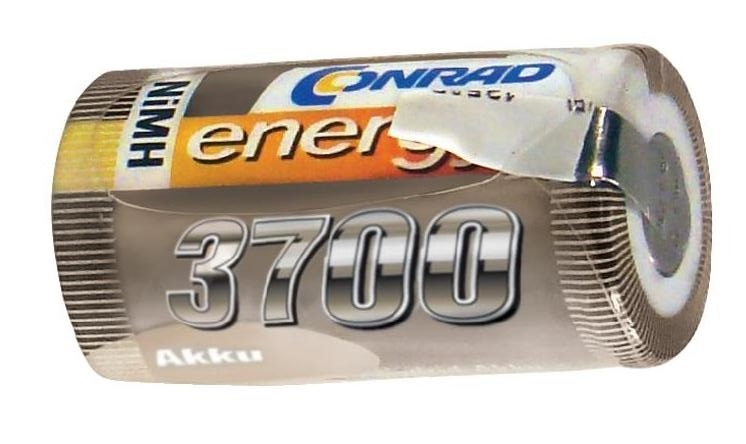
\includegraphics[width=0.6\linewidth]{img/3700}
\end{minipage}\hfill
\begin{minipage}{0.45\linewidth}
\centering 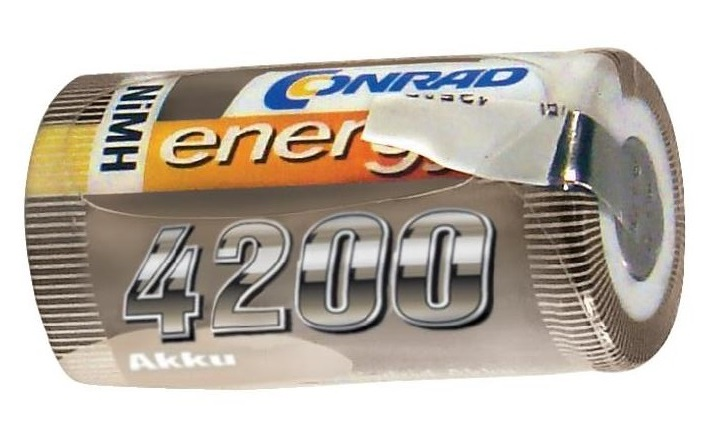
\includegraphics[width=0.6\linewidth]{img/4200}
\end{minipage}

Ces packs sont donc réalisés à partir d'accumulateurs montés en série. Il est alors possible de trouver les éléments suivants dans le commerce.

\begin{tabular}{|m{4cm}|m{3.5cm}|m{4cm}|m{3.5cm}|}
\hline
 &  & & \\
 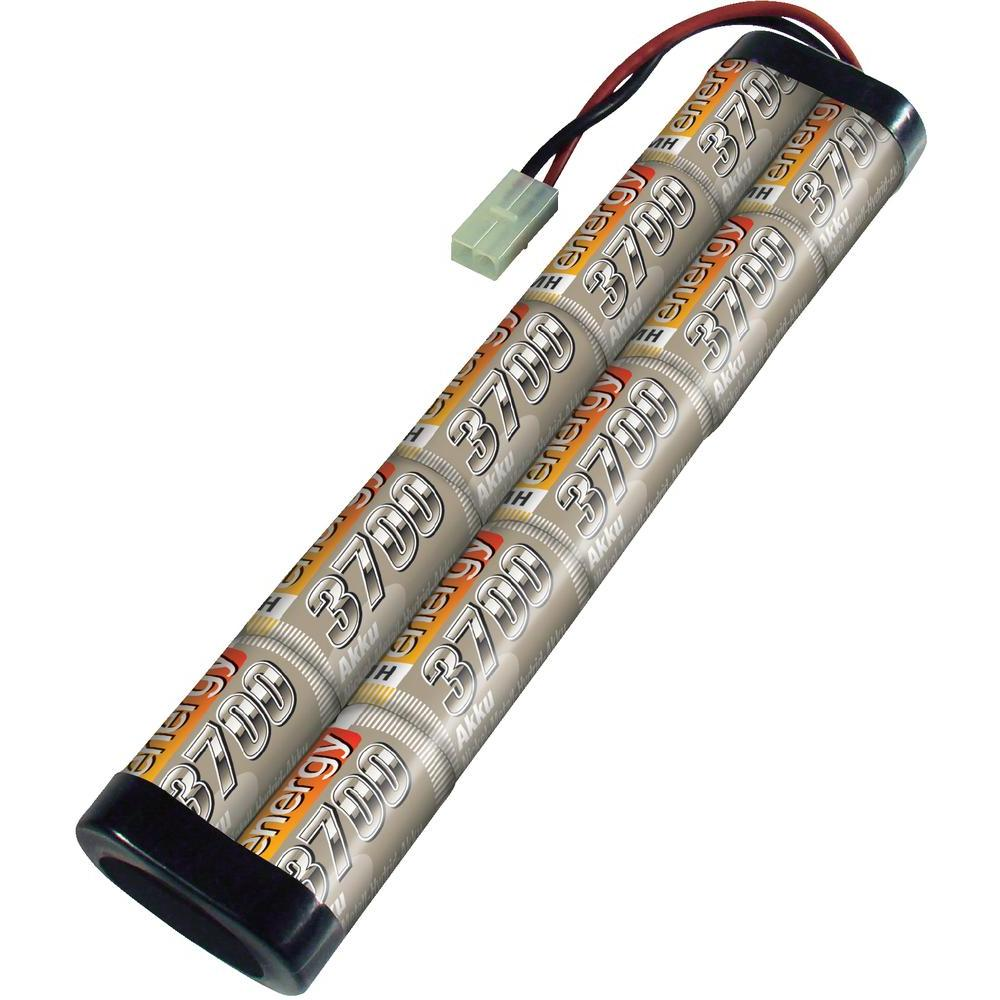
\includegraphics[width=4cm]{img/3700_10} & \begin{itemize}
 \item 10 accus  \item 3700mAh \item Total=12V  \end{itemize} & 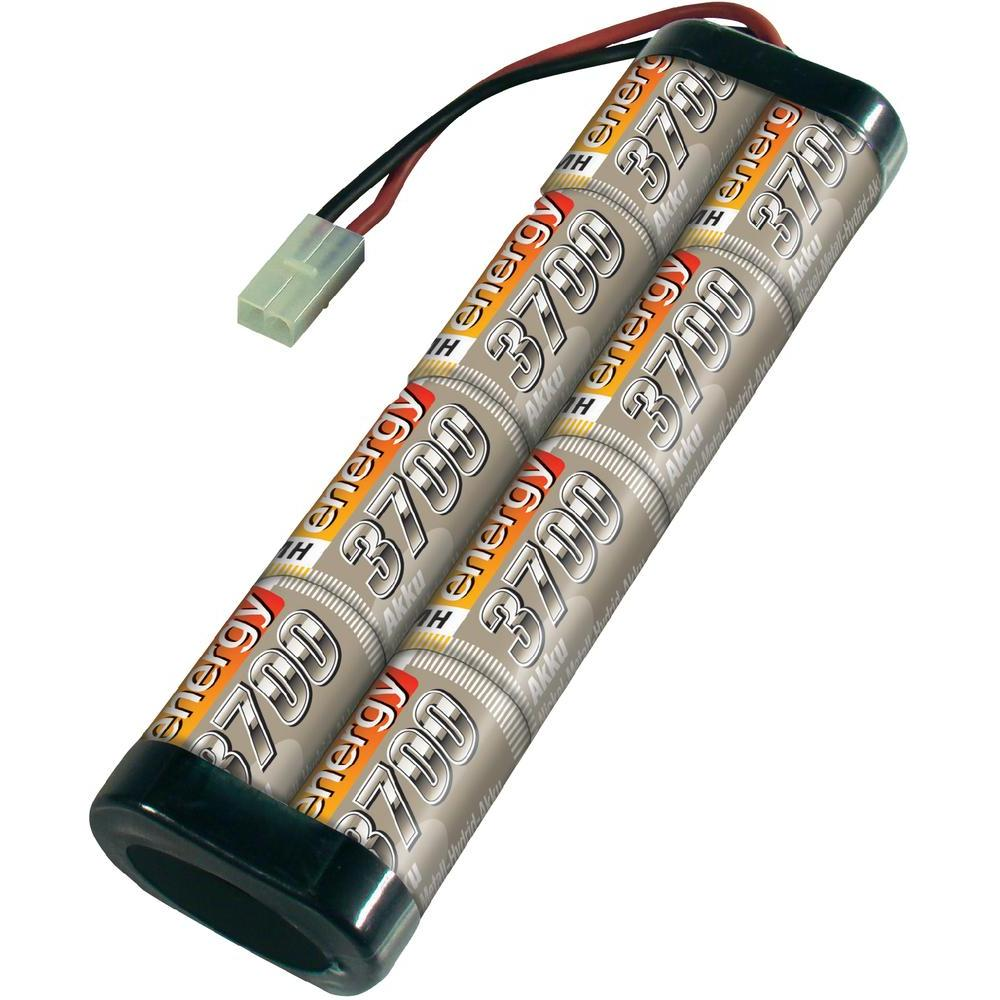
\includegraphics[width=4cm]{img/3700_8} & \begin{itemize}
 \item 8 accus  \item 3700mAh \item Total=9.6V  \end{itemize}  \\
\hline
 &  & & \\
 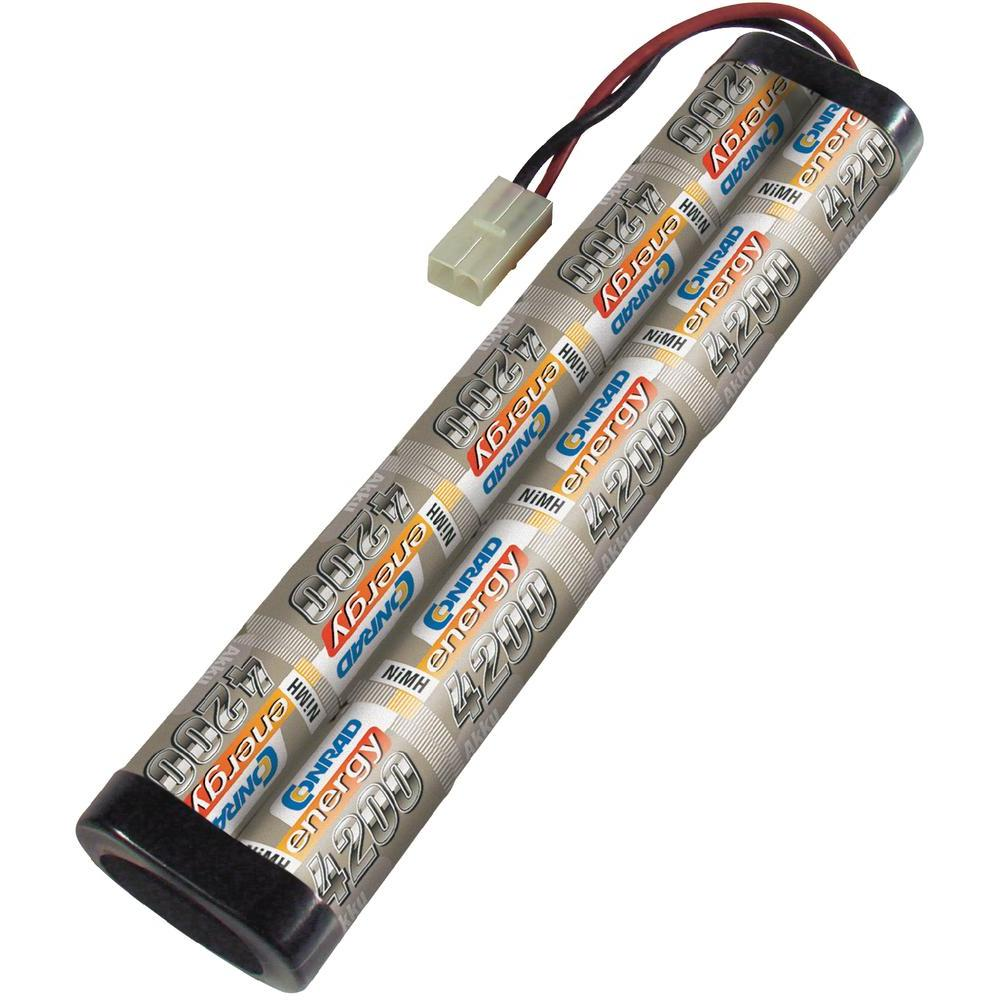
\includegraphics[width=4cm]{img/4200_10} & \begin{itemize}
 \item 10 accus  \item 4200mAh \item Total=12V  \end{itemize}  & 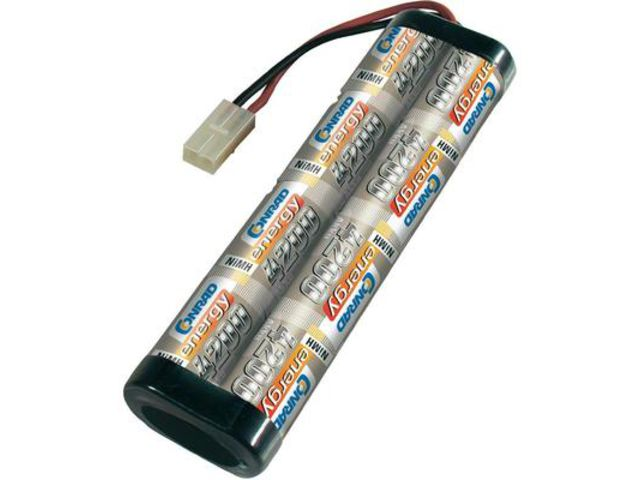
\includegraphics[width=4cm]{img/4200_8} & \begin{itemize}
 \item 8 accus  \item 4200mAh \item Total=9.6V  \end{itemize}  \\
\hline
 &  & & \\
 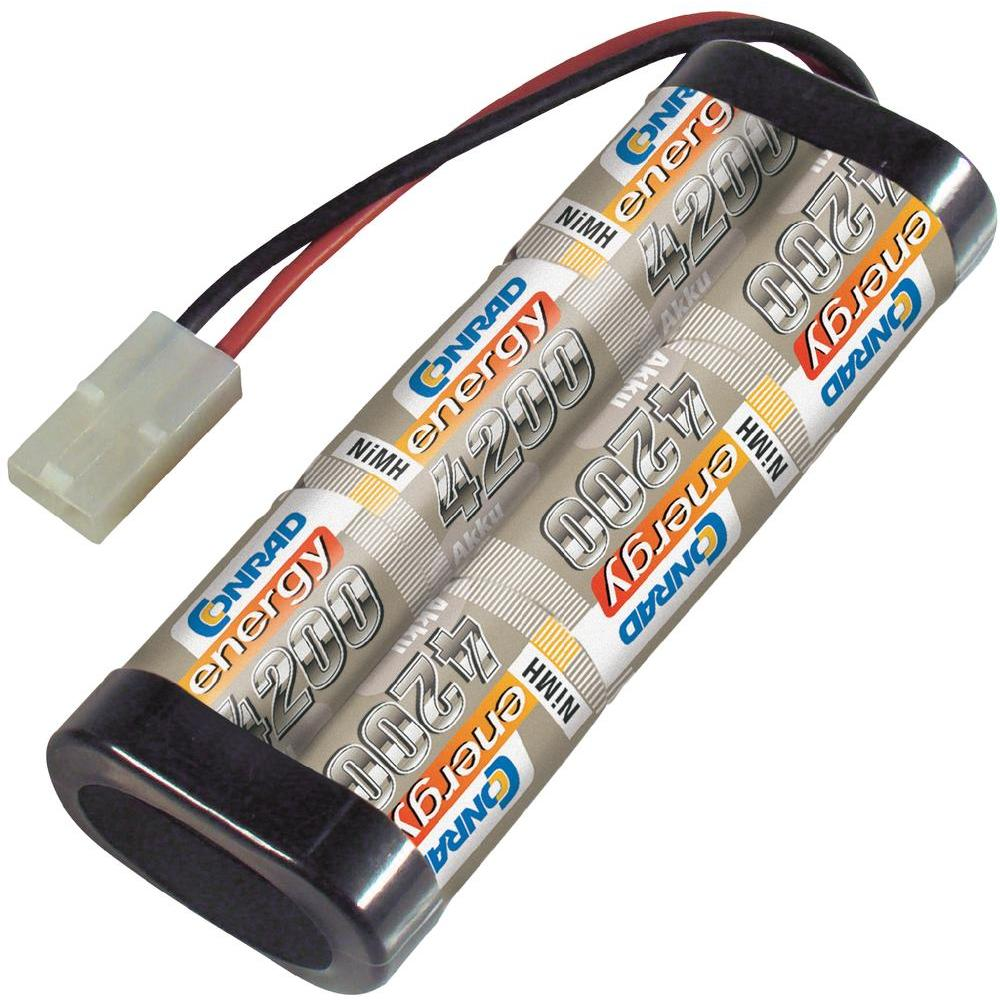
\includegraphics[width=4cm]{img/4200_6} & \begin{itemize}
 \item 6 accus  \item 4200mAh \item Total=7.2V  \end{itemize}  & 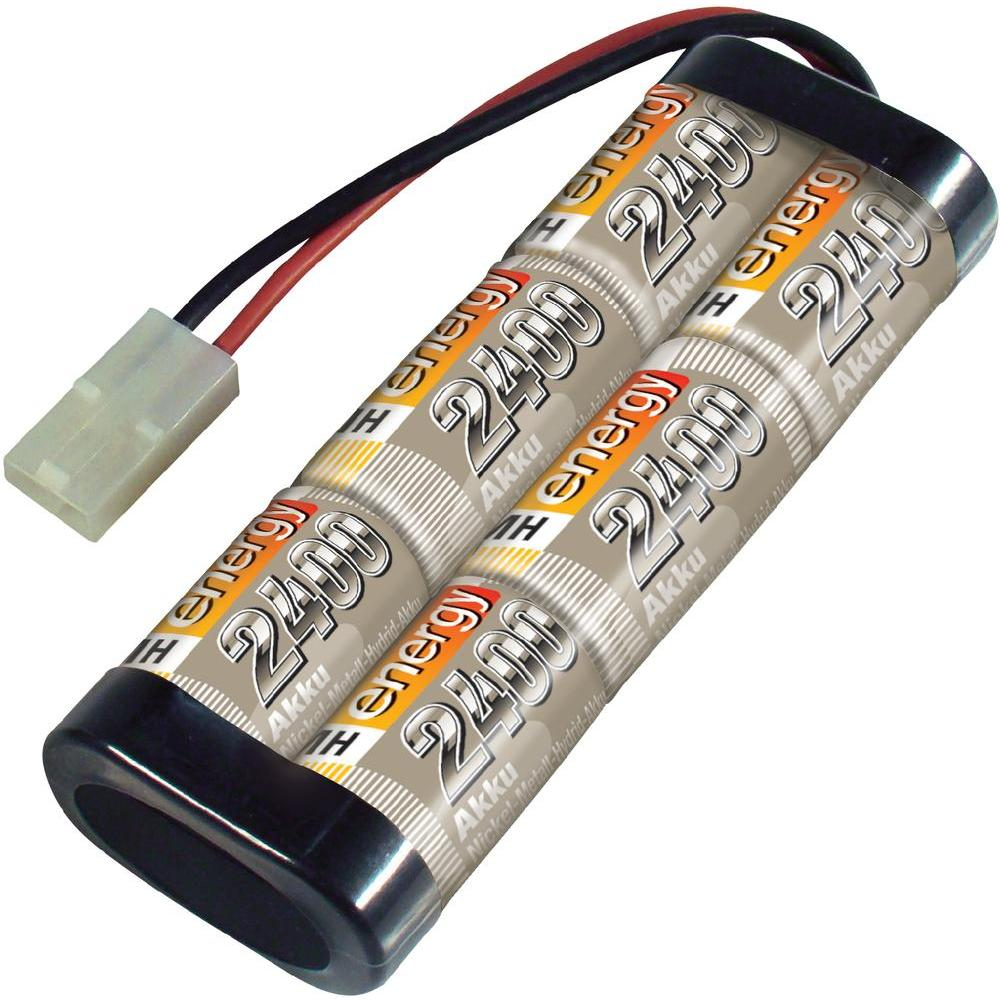
\includegraphics[width=4cm]{img/2400_6} & \begin{itemize}
 \item 6 accus  \item 2400mAh \item Total=7.2V  \end{itemize}  \\
\hline
\end{tabular}

\paragraph{Question 1:} Donner une relation entre le nombre d'accumulateurs et la tension de sortie du pack de batteries. Ce nombre joue-t-il sur la charge totale du pack ? Comment modifier cette charge ?

\paragraph{Question 2:} Calculez l'énergie (en Wh) stockée par chaque pack lorsqu'il est chargé.

~\

Un $Wh$ est équivalent à $3600J$.

\paragraph{Question 3:} Calculez l'énergie (en kJ) stockée par chaque pack lorsqu'il est chargé.

\paragraph{Question 4:} Le pack de 10 accumulateurs de 4200mAh est utilisé afin d'alimenter un système qui tire un courant de 2A. Combien de temps en théorie la batterie peut fournir une tension de 12V.

~\

La mise en parallèle de batteries permet de sommer leurs capacité. 

\paragraph{Question 5:} Combien de pack de batteries devront être mis en parallèle afin de garantir un fonctionnement durant 6h ?

\newpage

\section{Rhéostat de démarrage}

\subsection{Description du moteur à courant continu}

\begin{minipage}{0.65\linewidth}
Un \textbf{rhéostat de démarrage} permet de limiter l'intensité au démarrage en insérant des résistances au rotor qui sont éliminées progressivement une fois le moteur lancé. L'utilisation de ce type de démarreur n'est possible qu'avec les moteurs à rotor bobiné.

Ce type de montage était aussi installé sur les moteurs à excitation shunt, ce n'est pas le cas de l'exemple de l'exercice.

Dans le cadre de cet exercice, ce rhéostat a été mis en place afin de piloter un moteur de puissance faible.
\end{minipage}
 \hfill
\begin{minipage}{0.3\linewidth}
 \centering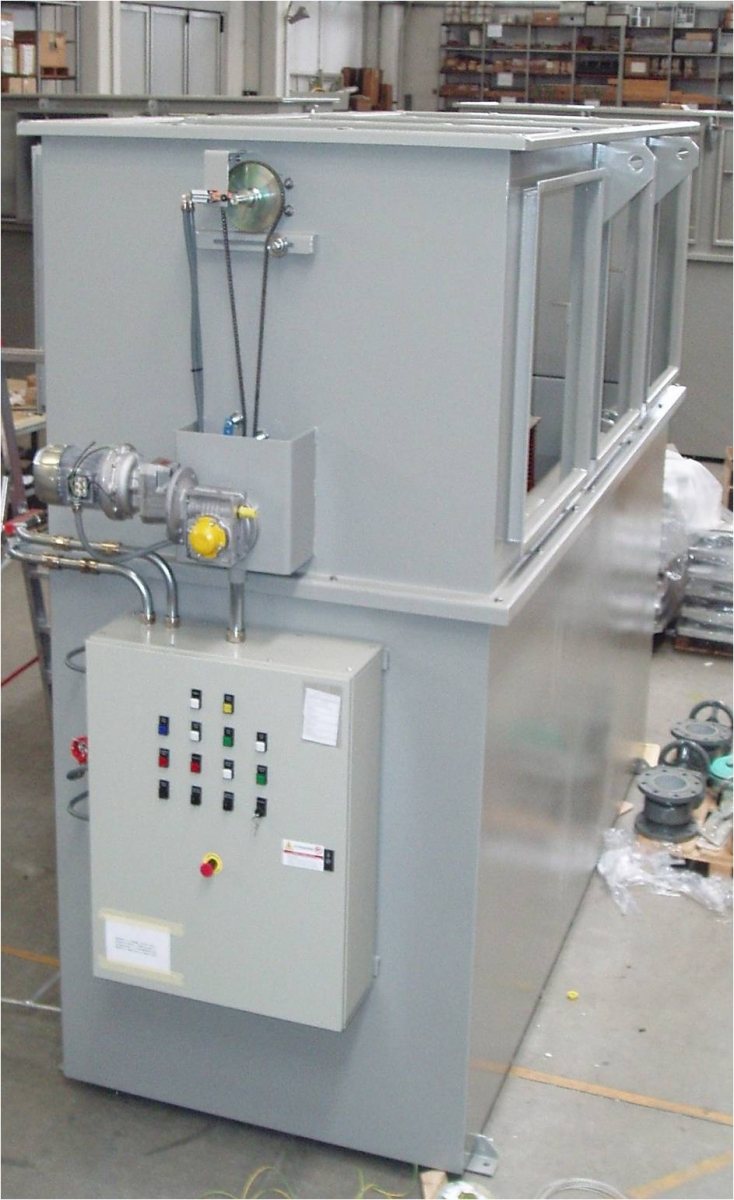
\includegraphics[width=0.5\linewidth]{img/rheostat}
\end{minipage}

\vspace{1cm}

\begin{minipage}{0.4\linewidth}
 \centering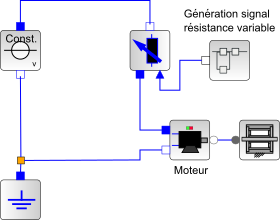
\includegraphics[width=0.9\linewidth]{img/Rheostat_xcos}
\end{minipage}
 \hfill
\begin{minipage}{0.55\linewidth}
Afin de modéliser le comportement de ce type de système, sur le schéma électrique suivant une résistance est placée en série avec un moteur électrique.

Un frein est placé à la suite du moteur électrique afin de simuler une résistance au démarrage ainsi que les différents frottements éventuels.
\end{minipage}

\vspace{1cm}

Ce modèle électrique a été simulé sur le logiciel Scilab-Xcos, des capteurs ont été ajoutés afin d'extraire les données suivantes:
\begin{itemize}
 \item Valeur de la résistance de pilotage (Ohm),
 \item Courant dans le circuit (A),
 \item Tension aux bornes de la résistance (V),
 \item Tension aux bornes du moteur (V),
 \item Vitesse du moteur (rad/s).
\end{itemize}

\begin{minipage}{0.4\linewidth}
Caractéristiques des composants:
\begin{itemize}
 \item $V_{in}=24V$,
 \item $r_{moteur}=2.07\Omega$,
 \item $L_{moteur}=0.62mH$,
 \item $K_c=5N.m.A^{-1}$,
 \item $J_{rotor}=3kg.m^2$,
 \item $f_{visqueux}=0.2N.m.rad^{-1}.s$,
 \item $f_{sec}=4N.m$,
 \item $R$ varie par palier (cf figure).
\end{itemize}
\end{minipage}
 \hfill
\begin{minipage}{0.59\linewidth}
	\begin{center}
	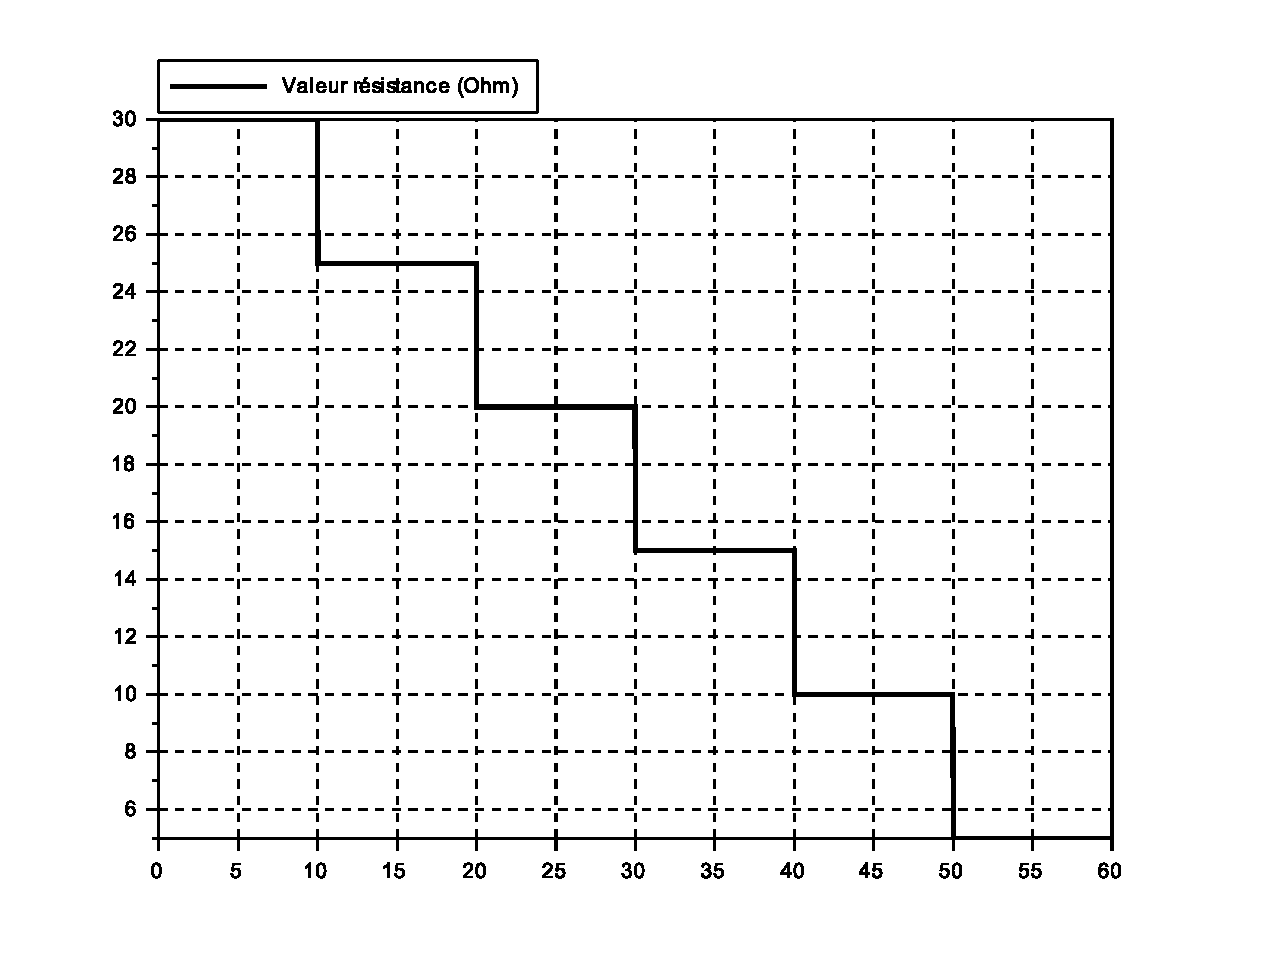
\includegraphics[width=0.8\linewidth]{img/Valeur_resistance}
	\end{center}
\end{minipage}

~\

\begin{center}
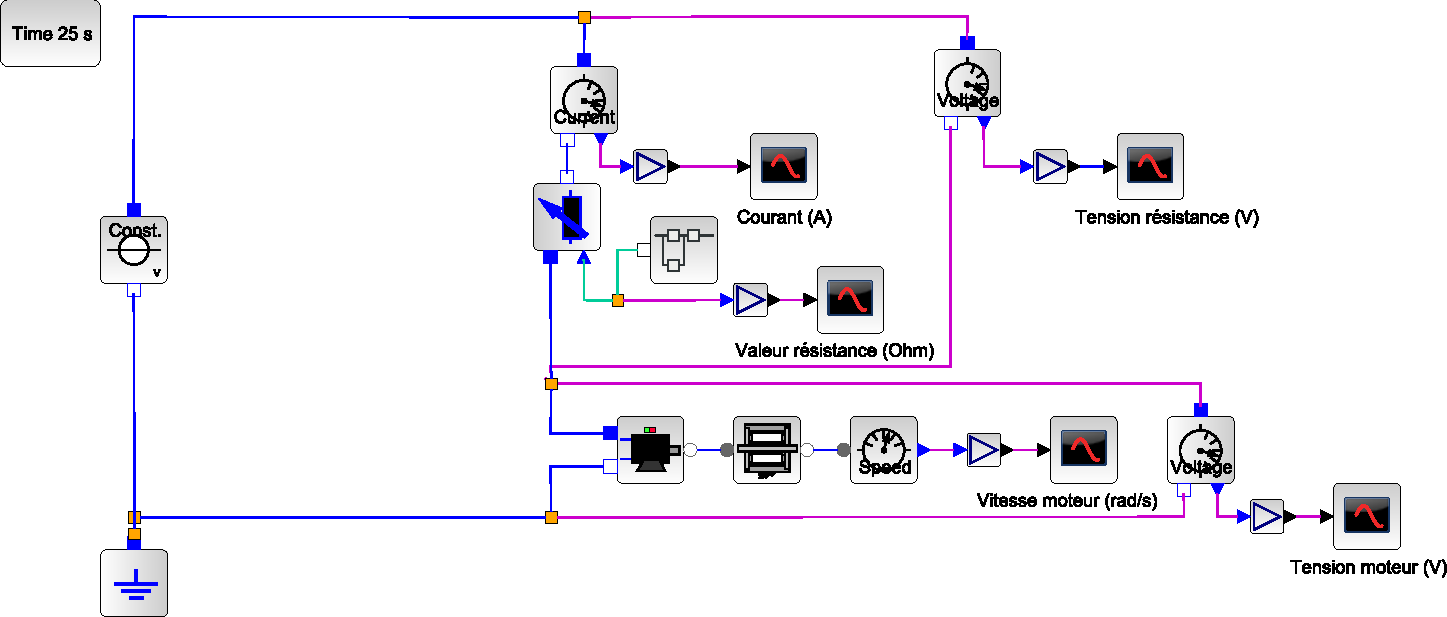
\includegraphics[width=0.9\linewidth]{img/Rheostat_capteurs_xcos}
\end{center}

~\

Les données extraites sont présentées sur les graphes suivants.

\begin{center}
	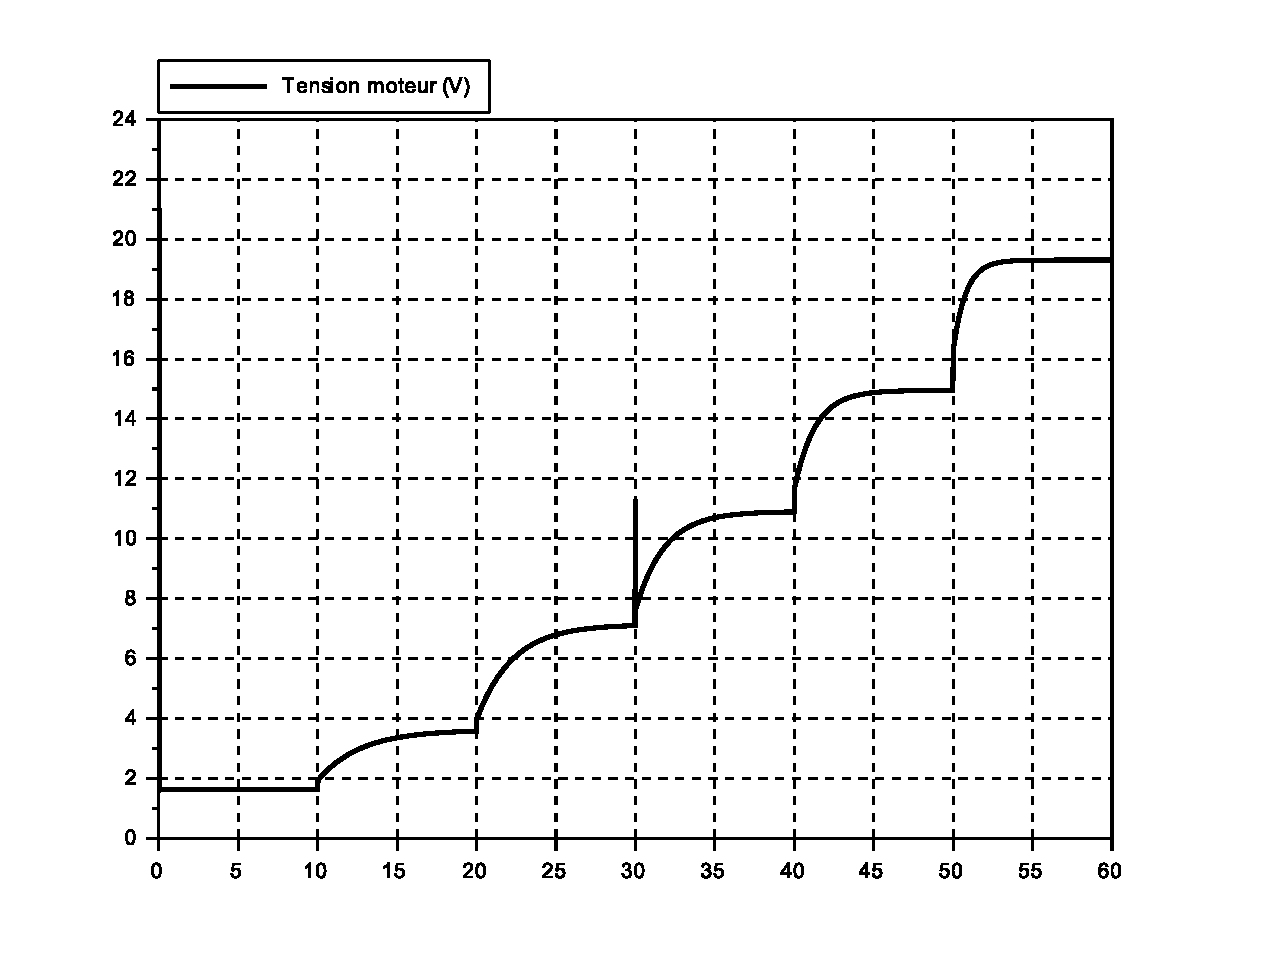
\includegraphics[width=0.9\linewidth]{img/Tension_moteur}
\end{center}

\begin{center}
	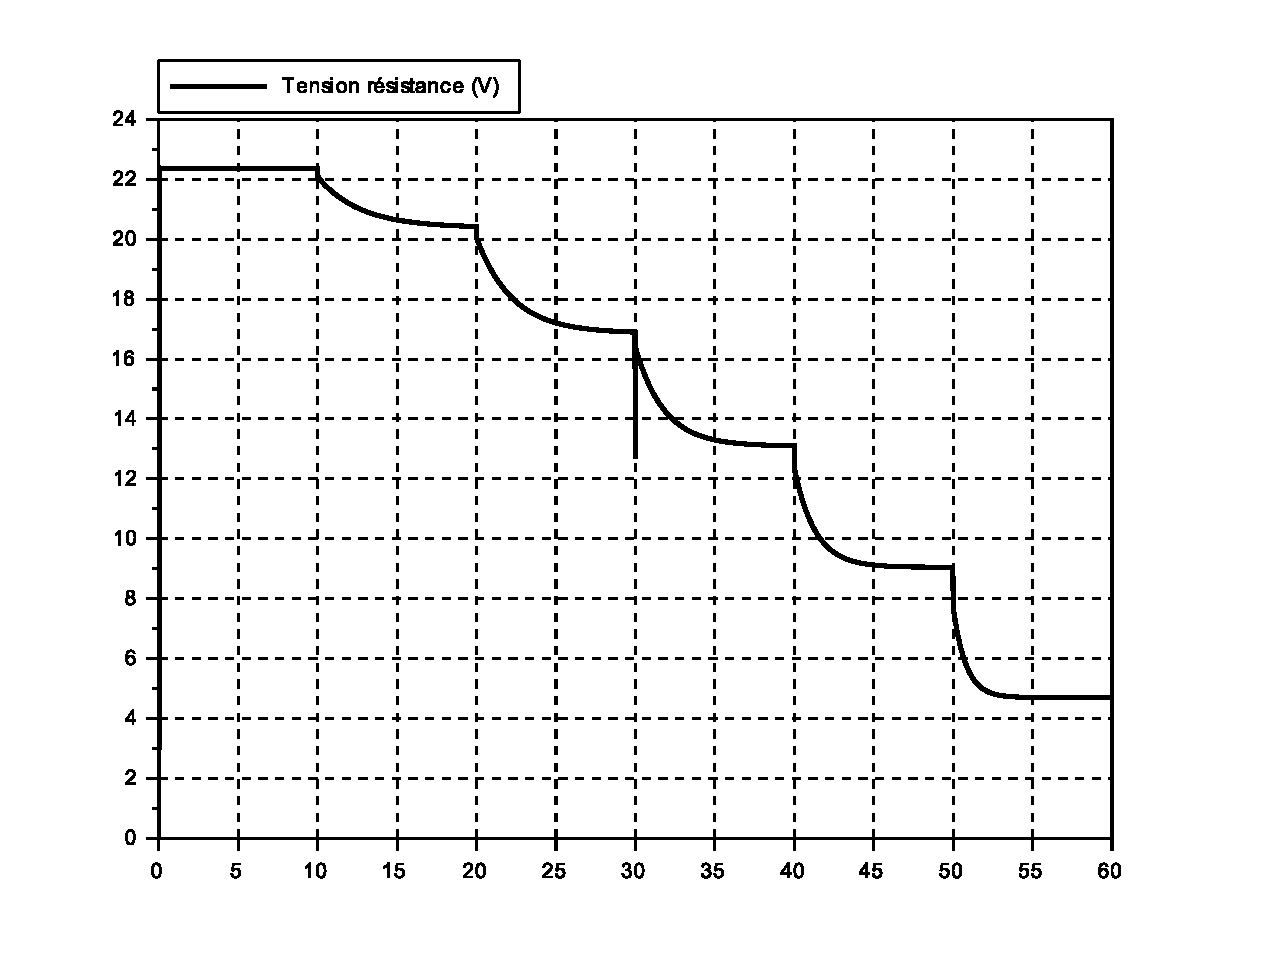
\includegraphics[width=0.9\linewidth]{img/Tension_resistance}
\end{center}

\begin{center}
	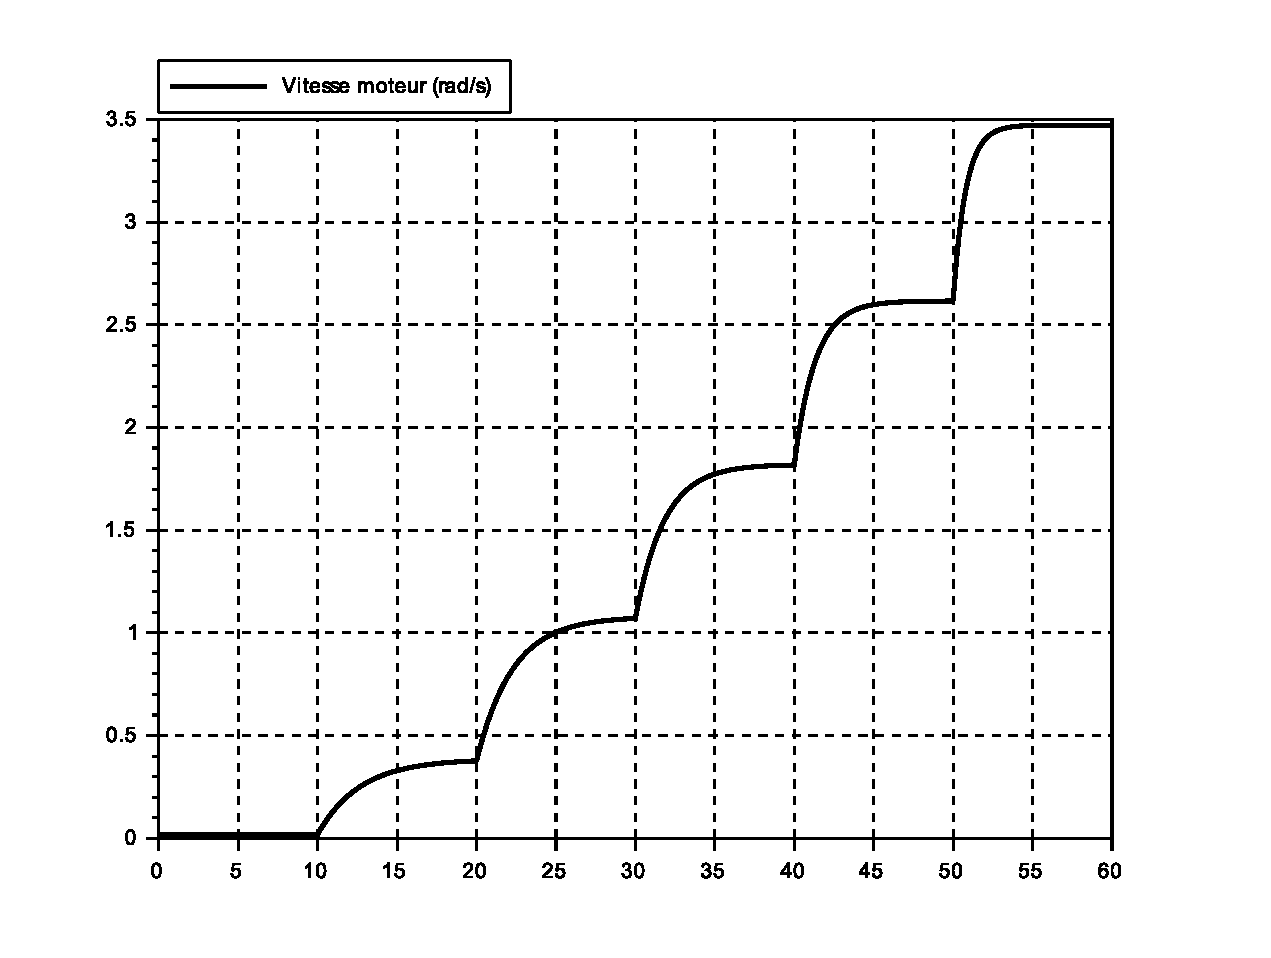
\includegraphics[width=0.9\linewidth]{img/Vitesse_moteur}
\end{center}

\begin{center}
	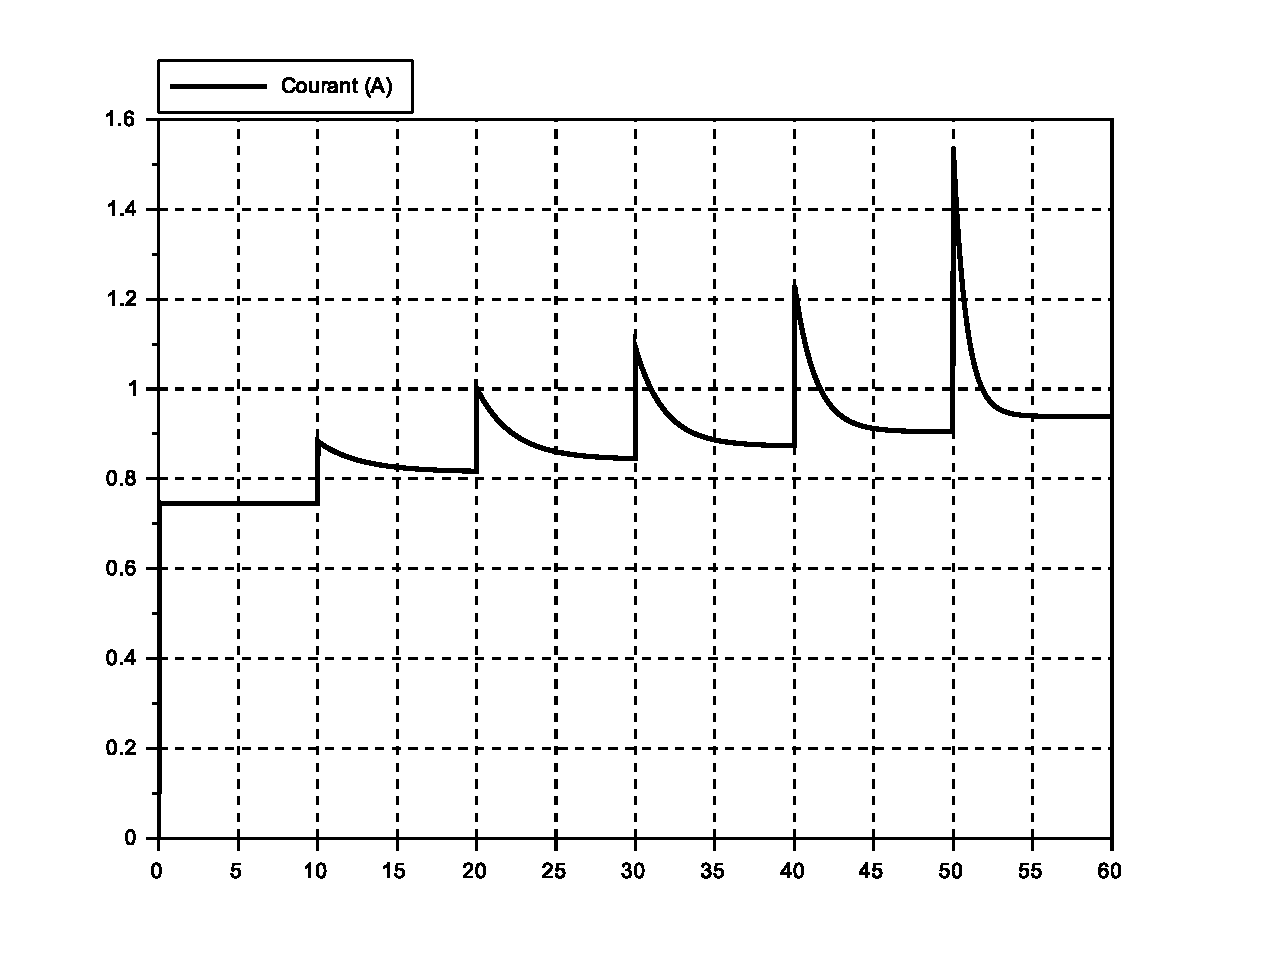
\includegraphics[width=0.9\linewidth]{img/Courant}
\end{center}

\paragraph{Question 1:} Déterminer à partir des courbes et de la valeur de la résistance interne du moteur $r_{moteur}$ la tension $U_r$ à ses bornes en régime établi pour chaque intervalle de temps. En relevant les valeurs de $U_m$, déterminer pour chaque intervalle la valeur de la force électromotrice $e$.

\paragraph{Question 2:} Relever la valeur de la vitesse du moteur pour chaque intervalle.

\paragraph{Question 3:} Quelle relation lie la vitesse du moteur et la force électromotrice ? En déduire, la valeur de la constante $K_e$. Cette valeur était-elle prévisible ?

\paragraph{Question 4:} Déterminer la puissance consommée par le moteur en régime établi et la tracer sur le graphe suivant.

\begin{center}
 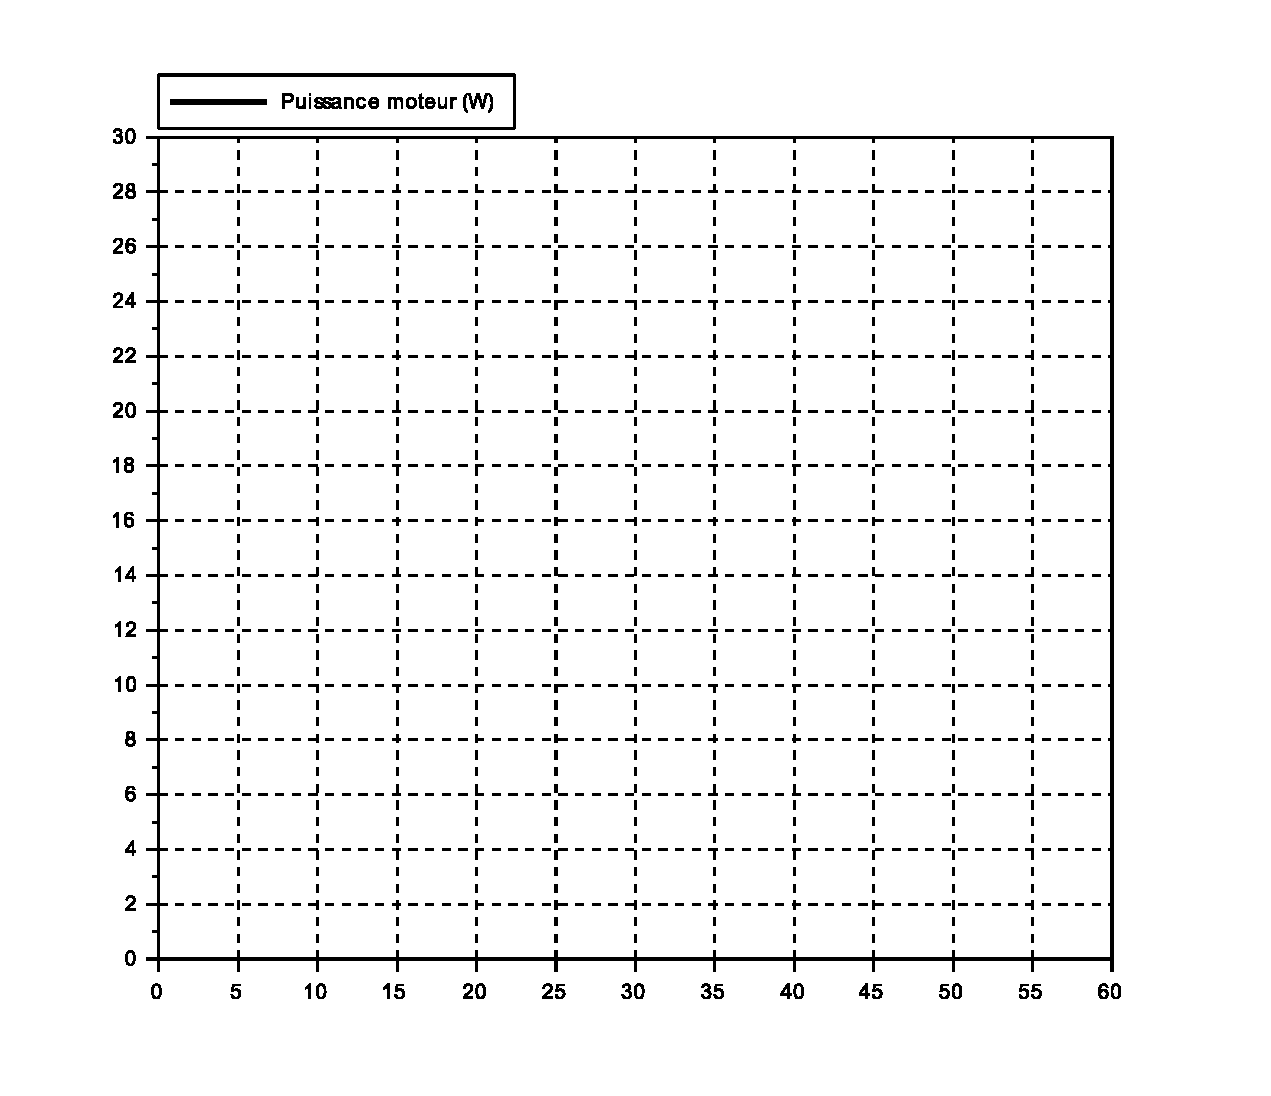
\includegraphics[width=0.8\linewidth]{img/Puissance_moteur_vide}
\end{center}

\paragraph{Question 5:} Déterminer la puissance fournie par l'alimentation en régime établi et la tracer sur le graphe suivant.

\begin{center}
 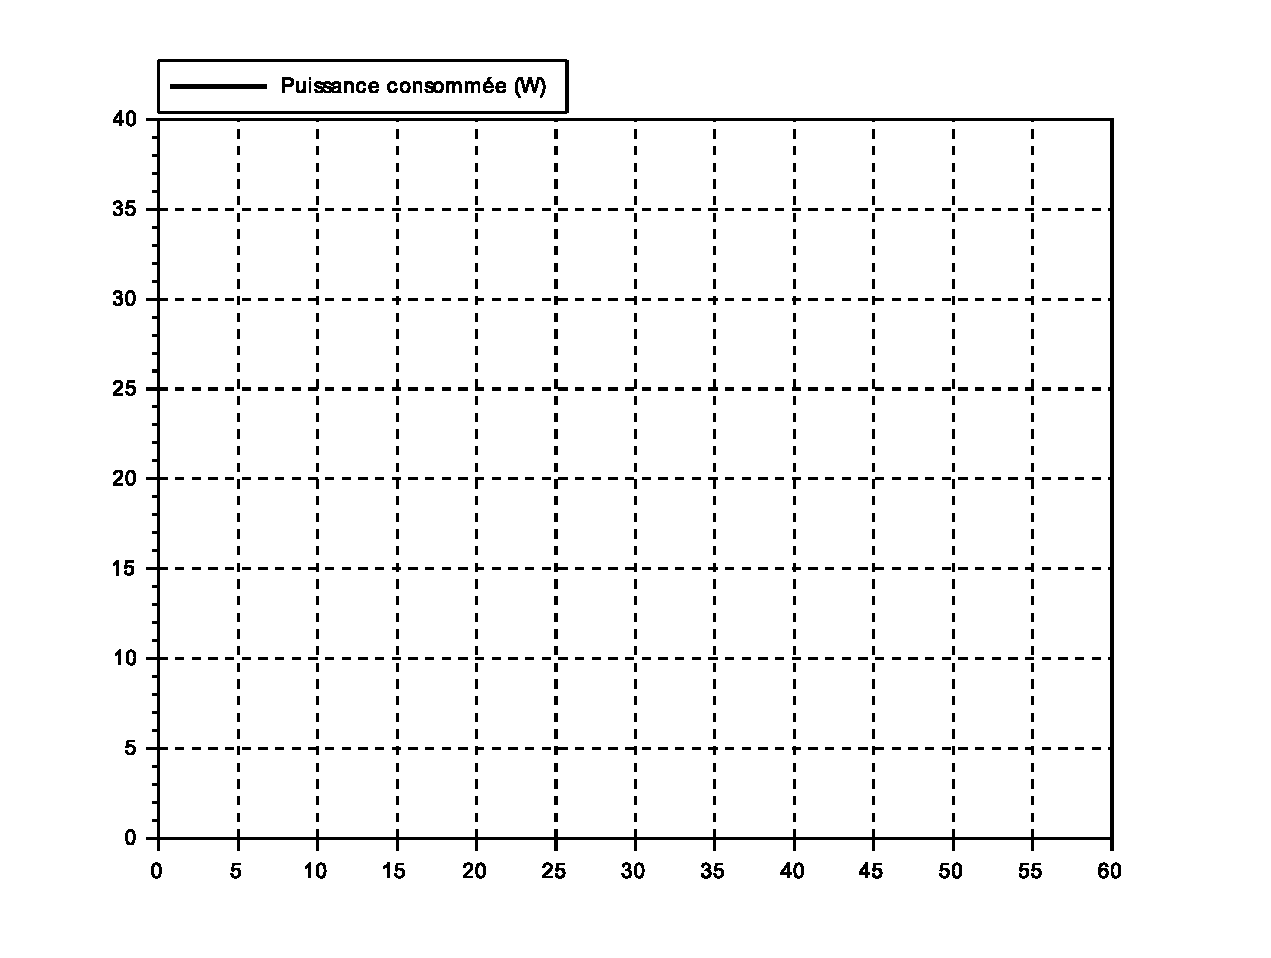
\includegraphics[width=0.8\linewidth]{img/Puissance_conso_vide}
\end{center}

\paragraph{Question 6:} Déterminer le rendement $\eta=\dfrac{P_{moteur}}{P_{fournie}}$ fournie par l'alimentation en régime établi et la tracer sur le graphe suivant

\begin{center}
 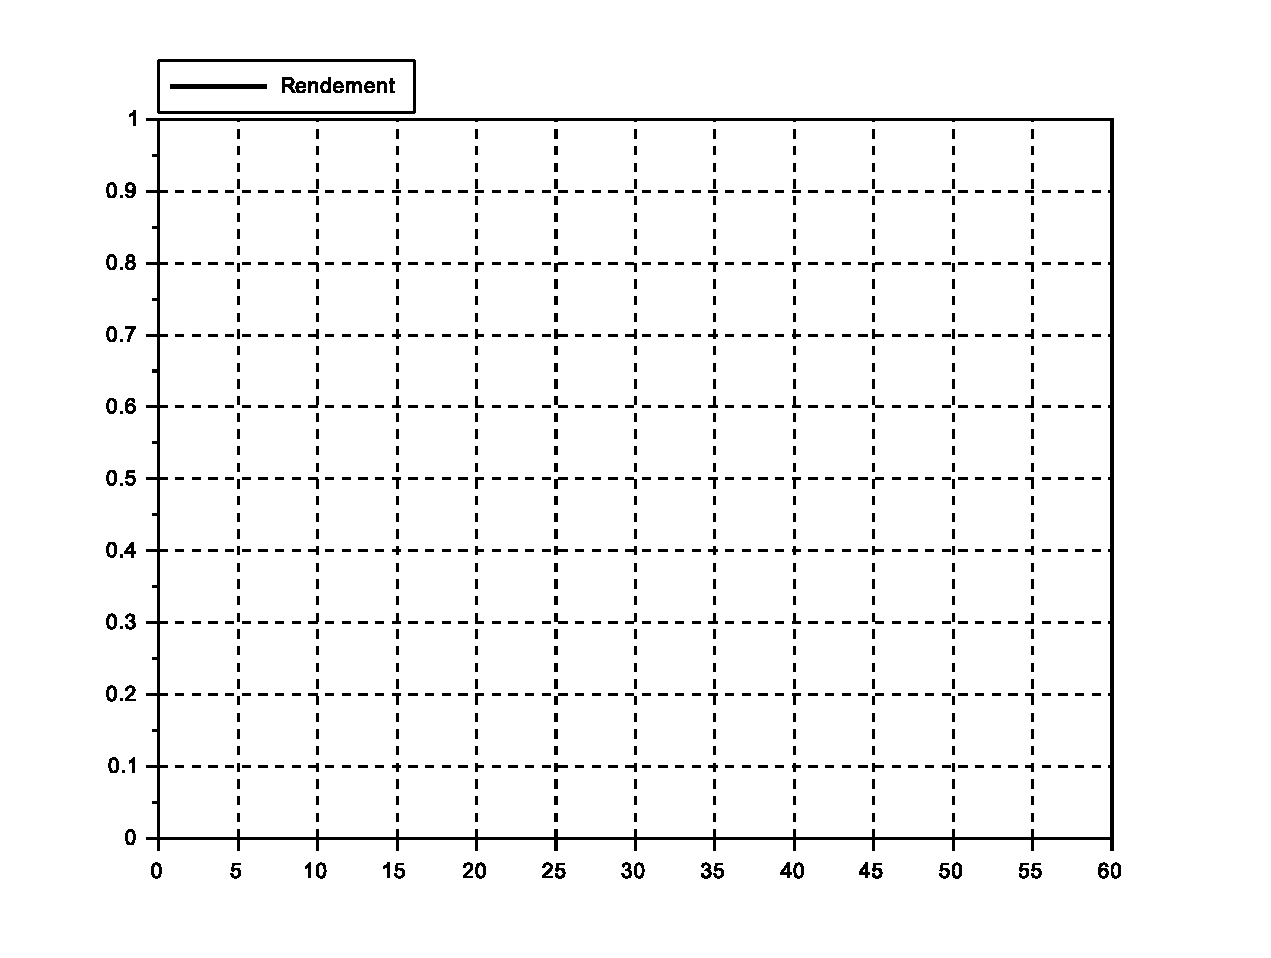
\includegraphics[width=0.8\linewidth]{img/Rendement_vide}
\end{center}

\paragraph{Question 7:} Proposer une critique de ce système à la vue du résultat précédent.

\newpage

\section{Flash d'appareil photo}

Le flash d'un appareil photo est effectué à partir d'un circuit électrique équivalent au suivant.

\begin{center}
 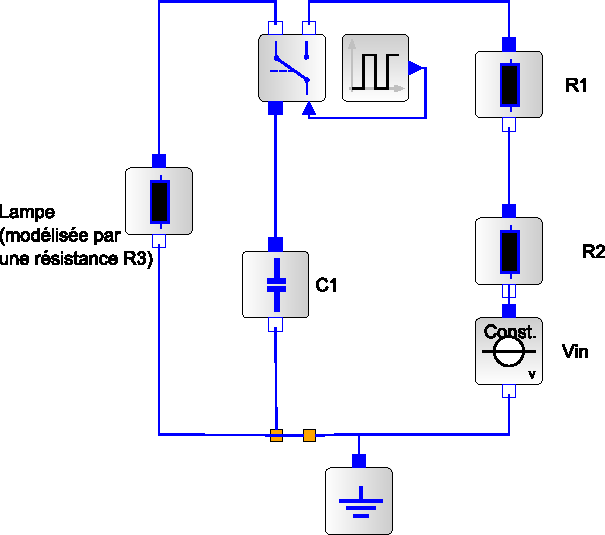
\includegraphics[width=0.5\linewidth]{img/Flash_xcos}
\end{center}

\begin{minipage}{0.4\linewidth}
Caractéristiques des composants:
\begin{itemize}
 \item $R_{1}=0.2k\Omega$,
 \item $R_{2}=0.6\Omega$,
 \item $R_{3}=0.1\Omega$,
 \item $C_{1}=3.3mF$,
 \item $V_{in}=6V$,
 \item Le basculement de l'interrupteur est donné ci-contre.
\end{itemize}
\end{minipage}
 \hfill
\begin{minipage}{0.59\linewidth}
	\begin{center}
	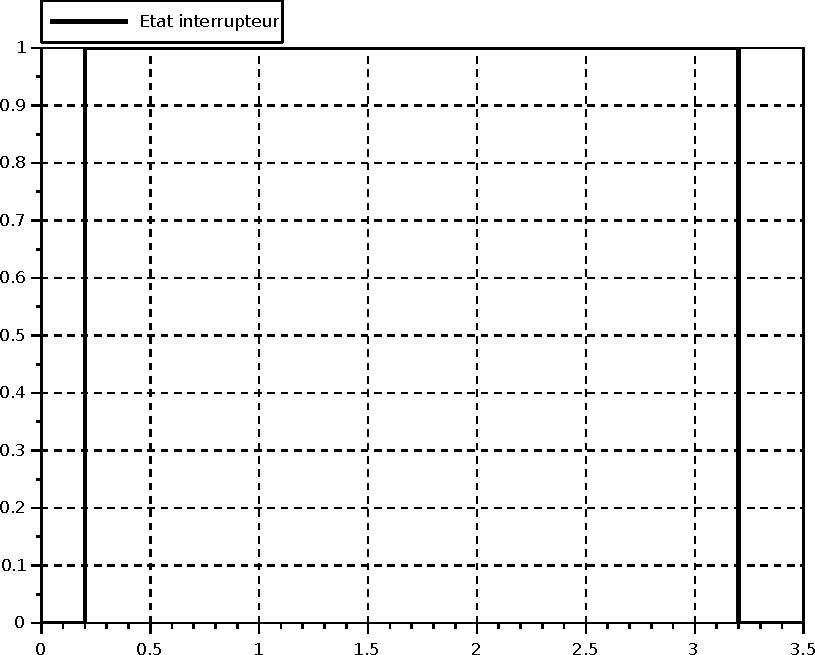
\includegraphics[width=0.8\linewidth]{img/Interrupteur}
	\end{center}
\end{minipage}

~\

\paragraph{Question 1:} Donner l'équation différentielle qui régit la charge du condensateur et en déduire le temps de charge nécessaire afin d'utiliser $95\%$ de la charge du condensateur.

\paragraph{Question 2:} Déterminer la réponse temporelle de cette charge.
 
Pour la suite, il sera considéré que le condensateur sera chargé à $100\%$ avant d'être utilisé.

\paragraph{Question 3:} Donner l'équation différentielle qui régit la décharge du condensateur dans la lampe et en déduire la durée de cette décharge jusqu'à ce qu'il ne reste que $5\%$ de la charge dans le condensateur.

\paragraph{Question 4:} Déterminer la réponse temporelle de cette décharge.

\paragraph{Question 5:} Compléter les diagrammes suivants.

\begin{center}
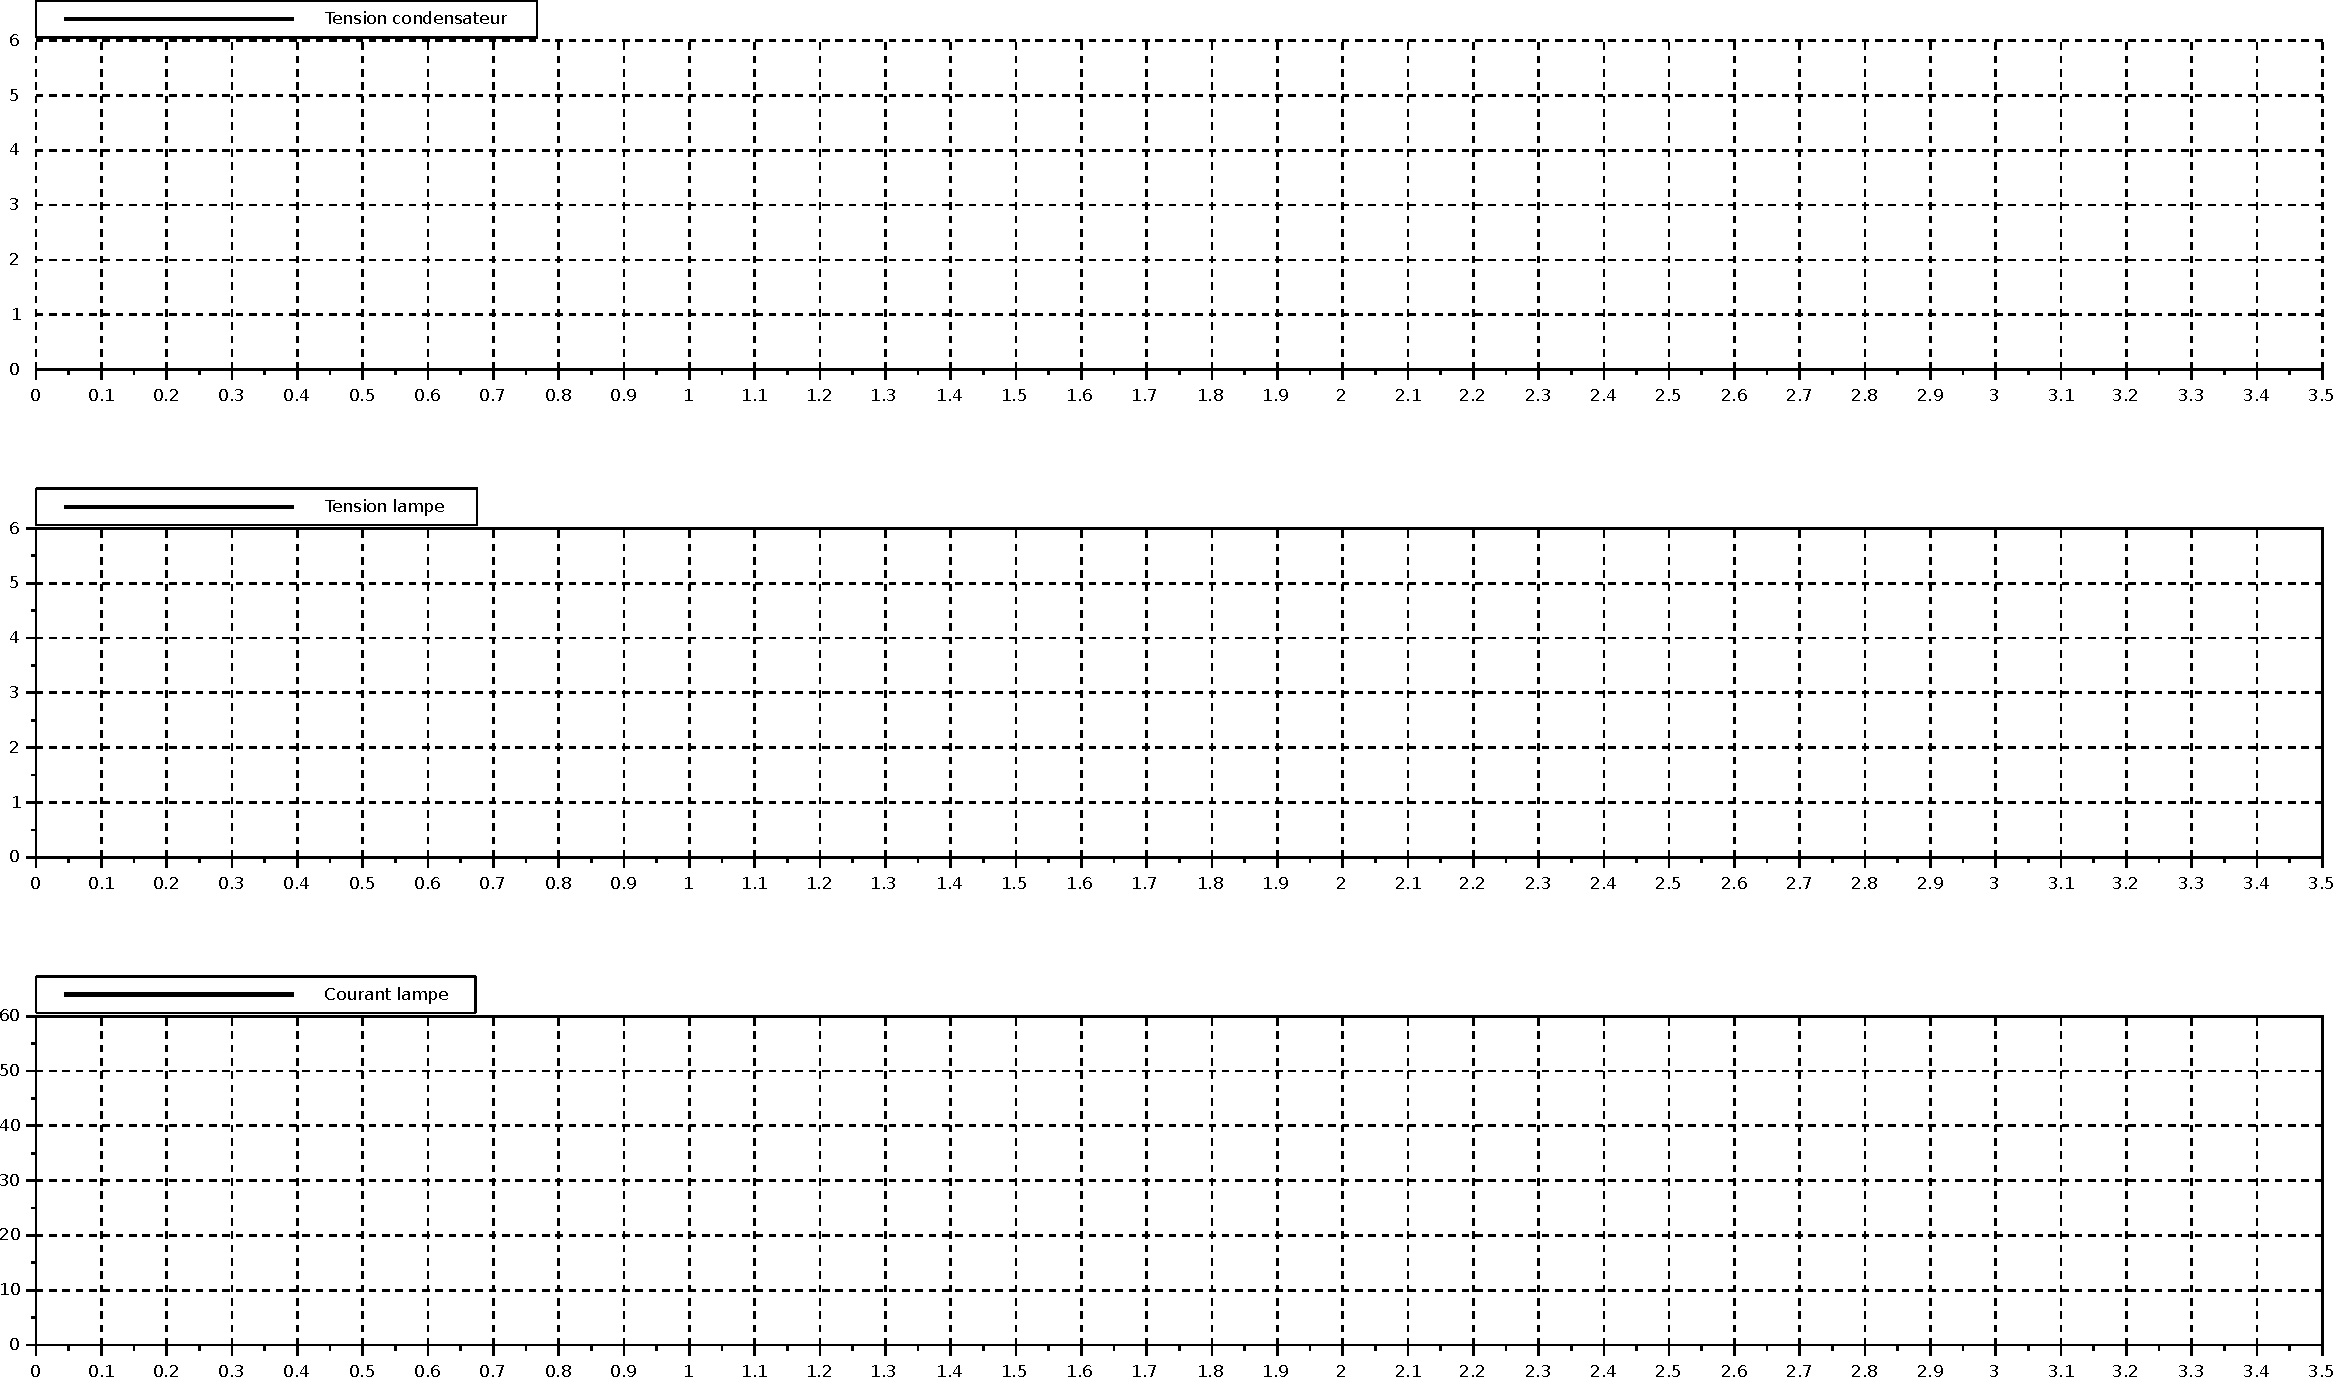
\includegraphics[width=0.9\linewidth]{img/Flash_results_vide}
\end{center}

\newpage

\section{Résistance de polarisation d'une DEL}

\begin{minipage}{0.6\linewidth}
Une diode électroluminescente doit être accompagnée d'une résistance de polarisation afin de fixer l'intensité du courant traversant la DEL $I_F$ à une
valeur proche de celle donnée par la documentation constructeur.

Nous souhaitons éclairer une DEL à partir d'une alimentation $V_in=+2.5V$.
\end{minipage}
\hfill
\begin{minipage}{0.39\linewidth}
\begin{center}
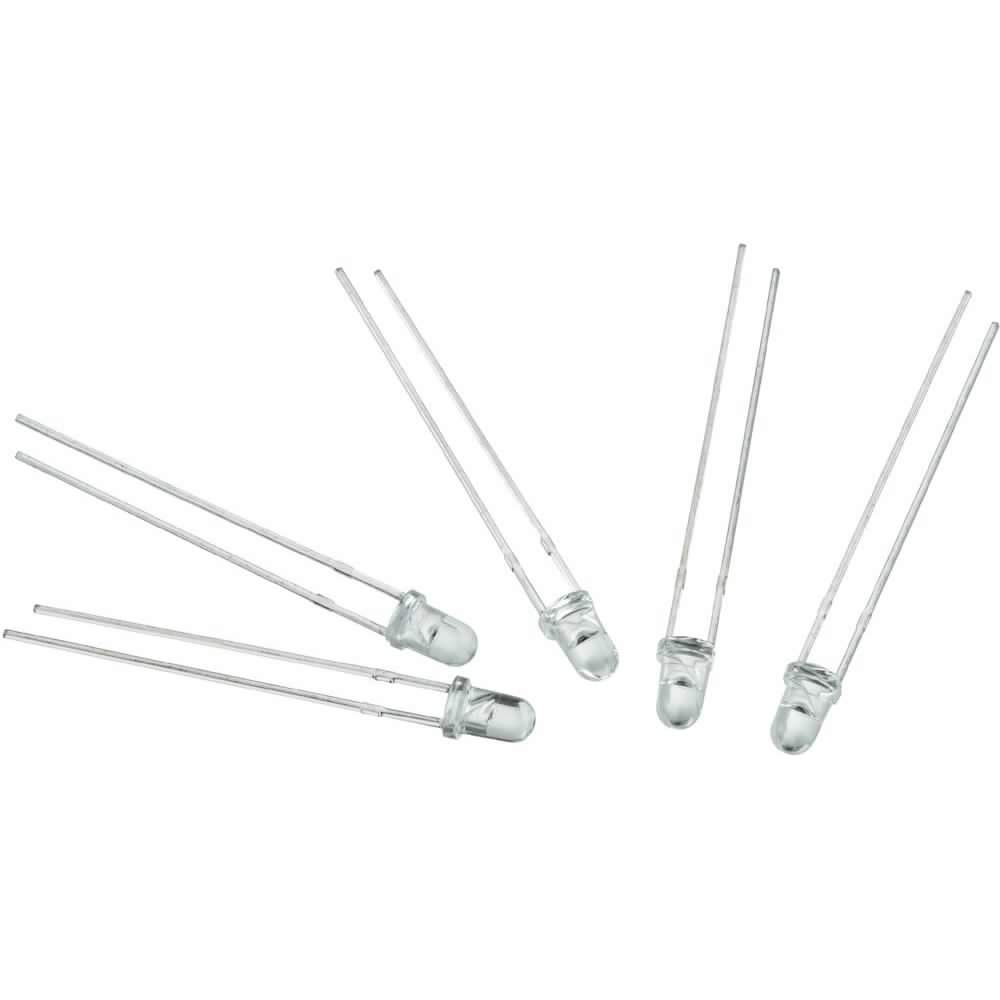
\includegraphics[width=0.9\linewidth]{img/DEL}
\end{center}
\end{minipage}

Pour cela, nous allons étudier le montage suivant.

\begin{center}
 \begin{circuitikz}[scale=2]
\ctikzset{bipoles/length=1.5cm}
\draw[color=bleuf] (2,0) -- (0,0) to[V, v=$u$] (0,2) to[R, l^=$R$] (2,2)  to[leDo, l^=$V_F$] (2,0);
\end{circuitikz}
\end{center}

Le constructeur donne les caractéristiques suivantes pour la DEL Everlight Opto 264-7UYC/S530-A2 jaune-orange ronde 3 mm 110 mcd 40° 10 mA 1.9V.

\begin{minipage}{0.49\linewidth}
\begin{center}
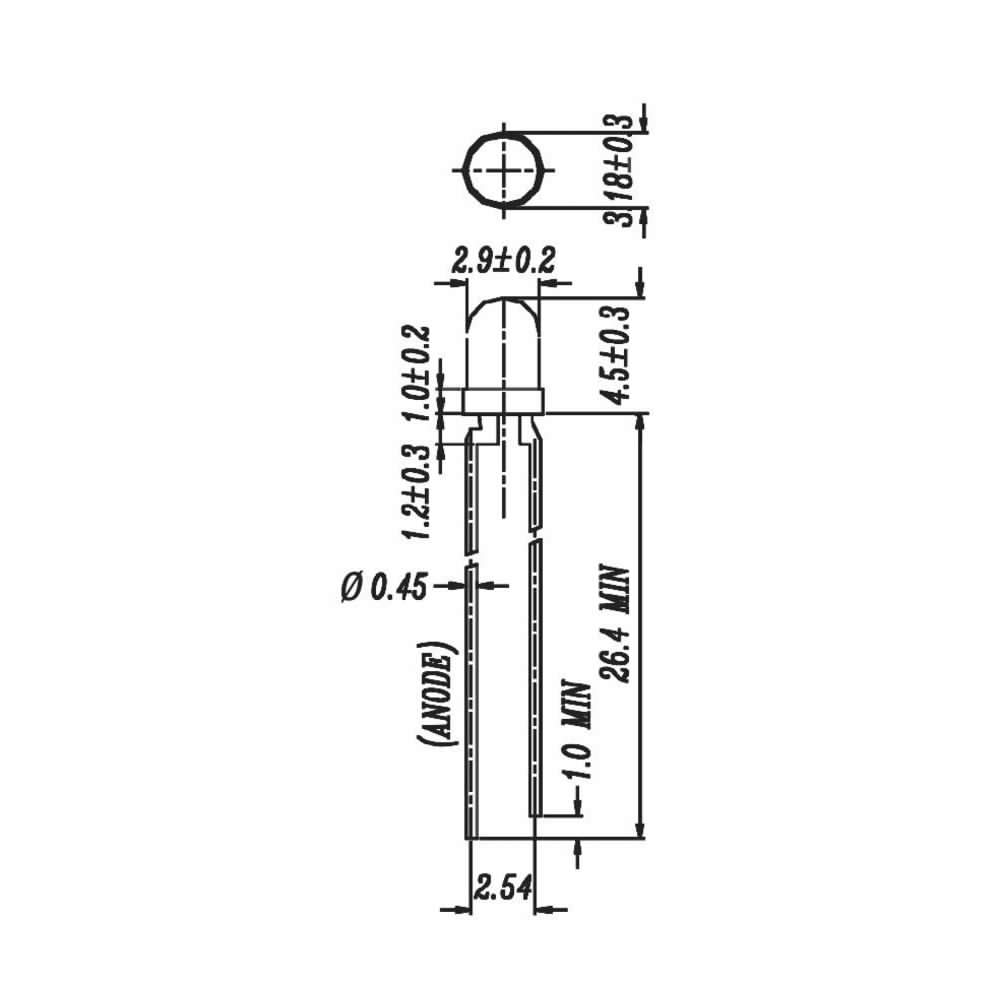
\includegraphics[width=0.7\linewidth]{img/DEL_data}
\end{center}
\end{minipage}
\hfill
\begin{minipage}{0.49\linewidth}
\begin{center}
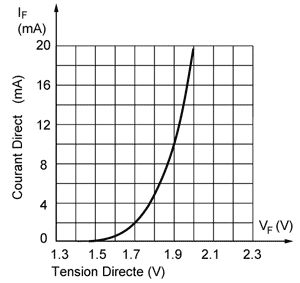
\includegraphics[width=0.7\linewidth]{img/DEL_carac}
\end{center}
\end{minipage}

Cette diode a été conçue pour travailler avec un courant $I_F=10mA$.

\paragraph{Question 1:} Donner la relation qui lie $i_R$ et $i_F$.

\paragraph{Question 2:} Donner la relation qui lie $U_R$ et $V_F$.

\paragraph{Question 3:} Donner la relation qui lie $U_R$ et $i_R$.

\paragraph{Question 4:} Écrire $i_F$ en fonction de $V_F$, $V_{in}$ et $R$. 

En superposant cette courbe à celle de la caractéristique de la DEL, le point de fonctionnement de la DEL apparaît à l'intersection des deux.

\paragraph{Question 5:} Superposer la courbe en question sur celle de la caractéristique de la DEL en faisant en sorte que le point de fonctionnement respecte les exigences du cahier des charges.

\paragraph{Question 6:} En déduire la valeur de la résistance $R$ à mettre en place.

\ifdef{\public}{\end{document}}

\newpage

\pagestyle{correction}

\section{Correction}

\subsection{Packs d'accumulateurs}
 
\paragraph{Question 1:} Donner une relation entre le nombre d'accumulateurs et la tension de sortie du pack de batteries. Ce nombre joue-t-il sur la charge totale du pack ? Comment modifier cette charge ?

$U_p=n.U_a$, avec $U_p$ tension du pack d'accumulateurs, $U_a$ tension d'un d'accumulateurs, $n$ nombre d'accumulateurs.

Le nombre d'accumulateurs ne joue pas sur la charge du pack. Il faut modifier la charge de l'accumulateur élémentaire afin de modifier la charge du pack.

\paragraph{Question 2:} Calculez l'énergie (en Wh) stockée par chaque pack lorsqu'il est chargé.

\begin{tabular}{|c|c|}
\hline
 44.4Wh & 35.52Wh \\
\hline
 50.4Wh & 40.32Wh \\
\hline
 30.24Wh & 17.28Wh \\
\hline
\end{tabular}

~\

Un $Wh$ est équivalent à $3600J$.

\paragraph{Question 3:} Calculez l'énergie (en kJ) stockée par chaque pack lorsqu'il est chargé.

\begin{tabular}{|c|c|}
\hline
 159.84kJ & 127.87kJ \\
\hline
181.44kJ & 145.15kJ \\
\hline
108.86kJ & 62.2kJ \\
\hline
\end{tabular}

\paragraph{Question 4:} Le pack de 10 accumulateurs de 4200mAh est utilisé afin d'alimenter un système qui tire un courant de 2A. Combien de temps en théorie la batterie peut fournir une tension de 12V.

En considérant une tension constante durant toute la décharge de la batterie, on trouve $T=\dfrac{4.2Ah}{2A}=2.1h=2h6min$.

~\

La mise en parallèle de batteries permet de sommer leurs capacité. 

\paragraph{Question 5:} Combien de pack de batteries devront être mis en parallèle afin de garantir un fonctionnement durant 6h ?

Il faut alors mettre 3 packs en parallèle.

\subsection{Rhéostat de démarrage}

\paragraph{Question 1:}

La tension aux bornes du moteur est $U_m=U_r+U_L+e$, avec $U_L=0$ en régime établi. De plus, la loi des mailles donne $U_{in}=U_R+U_m$

Calcul de $U_r$ à partir de $i$ et de $r_{moteur}$. Mesure de $U_m$, et calcul de $e$.

\begin{enumerate}
 \item $0<t<4s$: $U_r=0.75*2.07=1.55$, $U_m=1.7$, $e=0.15$
 \item $4<t<8s$: $U_r=0.82*2.07=1.7$, $U_m=3.6$, $e=1.9$
 \item $8<t<12s$: $U_r=0.85*2.07=1.76$, $U_m=7$, $e=5.24$
 \item $12<t<16s$: $U_r=0.87*2.07=1.8$, $U_m=10.9$, $e=9.1$
 \item $16<t<20s$: $U_r=0.9*2.07=1.86$, $U_m=15$, $e=13.14$
 \item $20<t<25s$: $U_r=0.94*2.07=1.94$, $U_m=19.4$, $e=17.46$
\end{enumerate}

\paragraph{Question 2:}

Relevé de la vitesse du moteur.

\begin{enumerate}
 \item $0<t<10s$: $\Omega_m=0.016$
 \item $10<t<20s$: $\Omega_m=0.37$
 \item $20<t<30s$: $\Omega_m=1.1$
 \item $30<t<40s$: $\Omega_m=1.82$
 \item $40<t<50s$: $\Omega_m=2.62$
 \item $60<t<60s$: $\Omega_m=3.47$
\end{enumerate}

\paragraph{Question 3:}

\begin{center}
 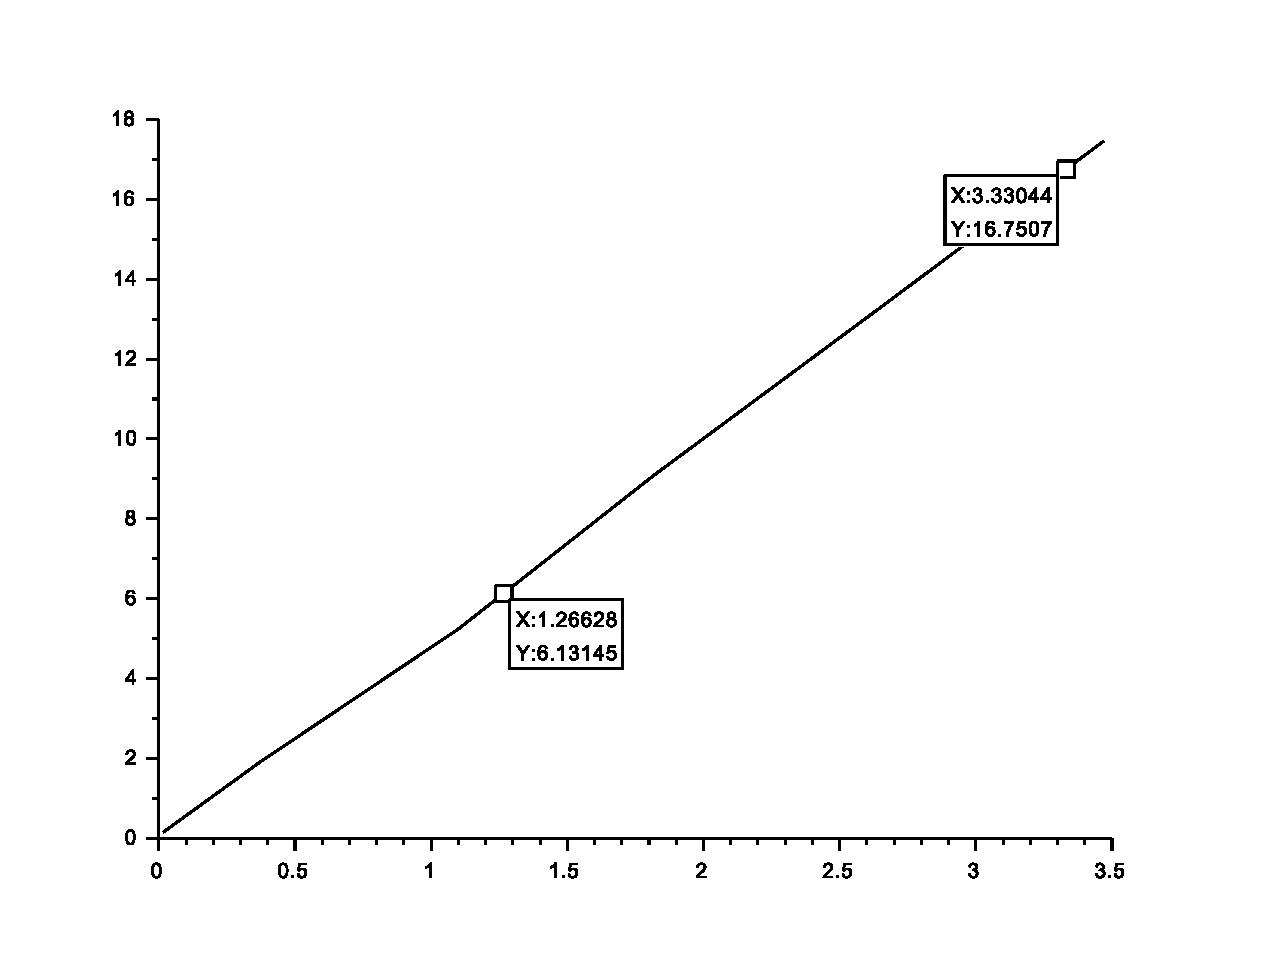
\includegraphics[width=0.8\linewidth]{img/calcul_ke}
\end{center}

Point 1: $16.75=a*3.33+b$
Point 2: $6.13=a*1.27+b$

Taux d'accroissement: $16.75-6.13/(3.33-1.27)=5.15$

On trouve une constante de vitesse environ égale à $K_c=5$.

\paragraph{Question 4:}

\begin{center}
 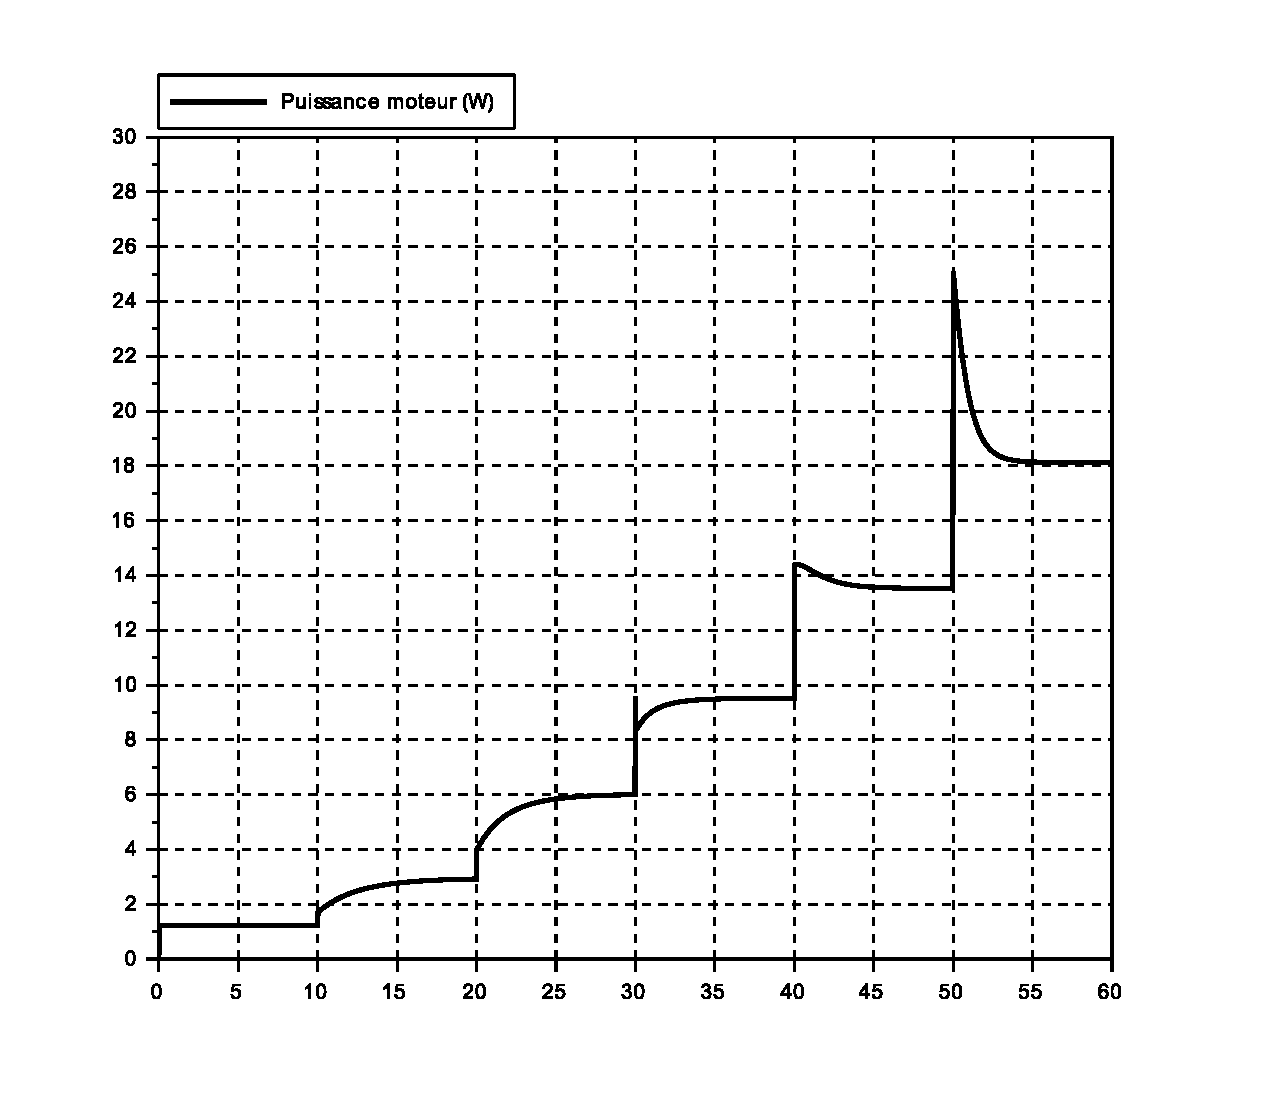
\includegraphics[width=0.8\linewidth]{img/Puissance_moteur}
\end{center}

\paragraph{Question 5:}

\begin{center}
 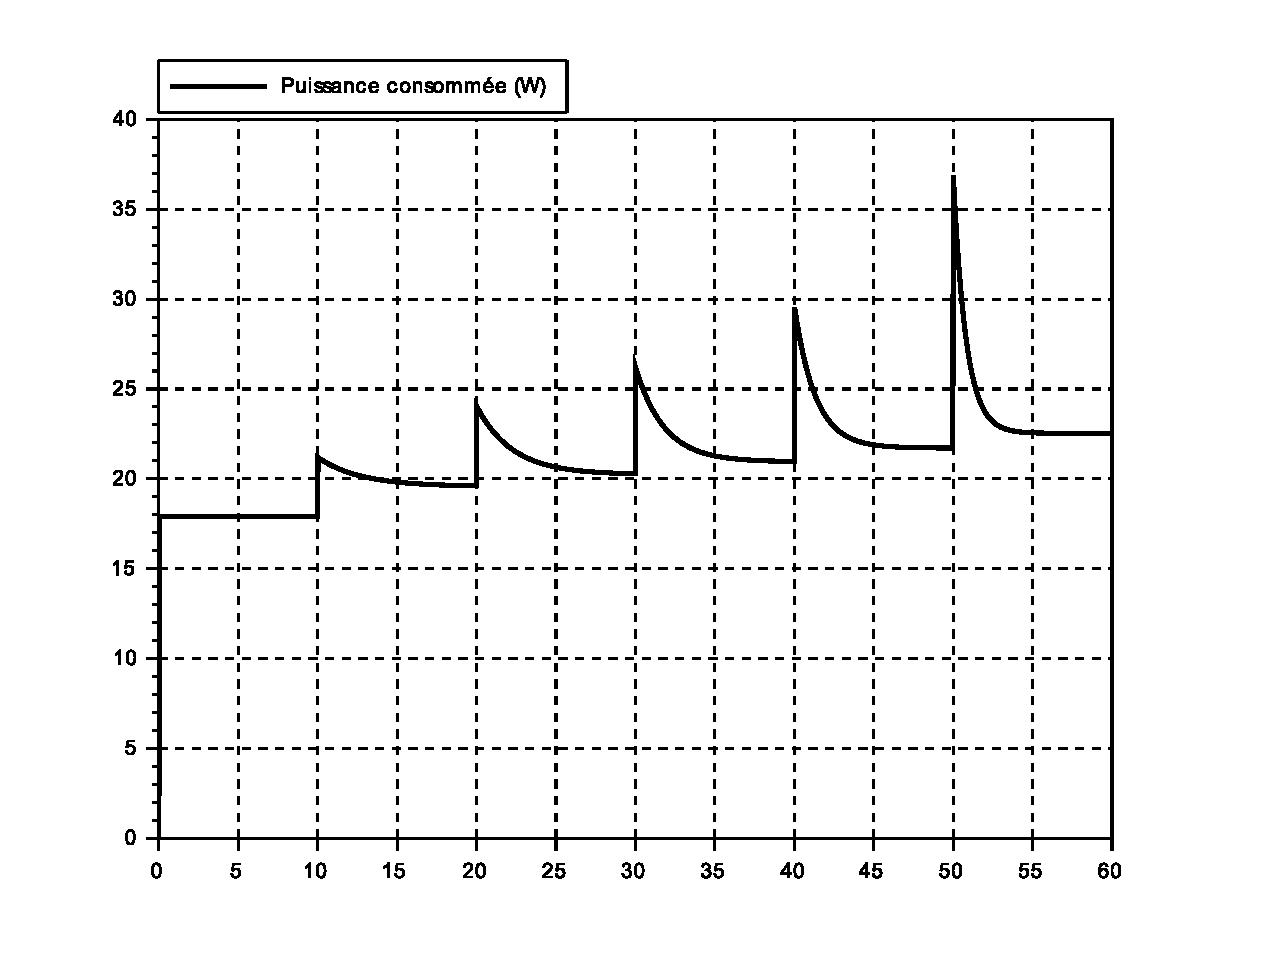
\includegraphics[width=0.8\linewidth]{img/Puissance_conso}
\end{center}

\paragraph{Question 6:}

\begin{center}
 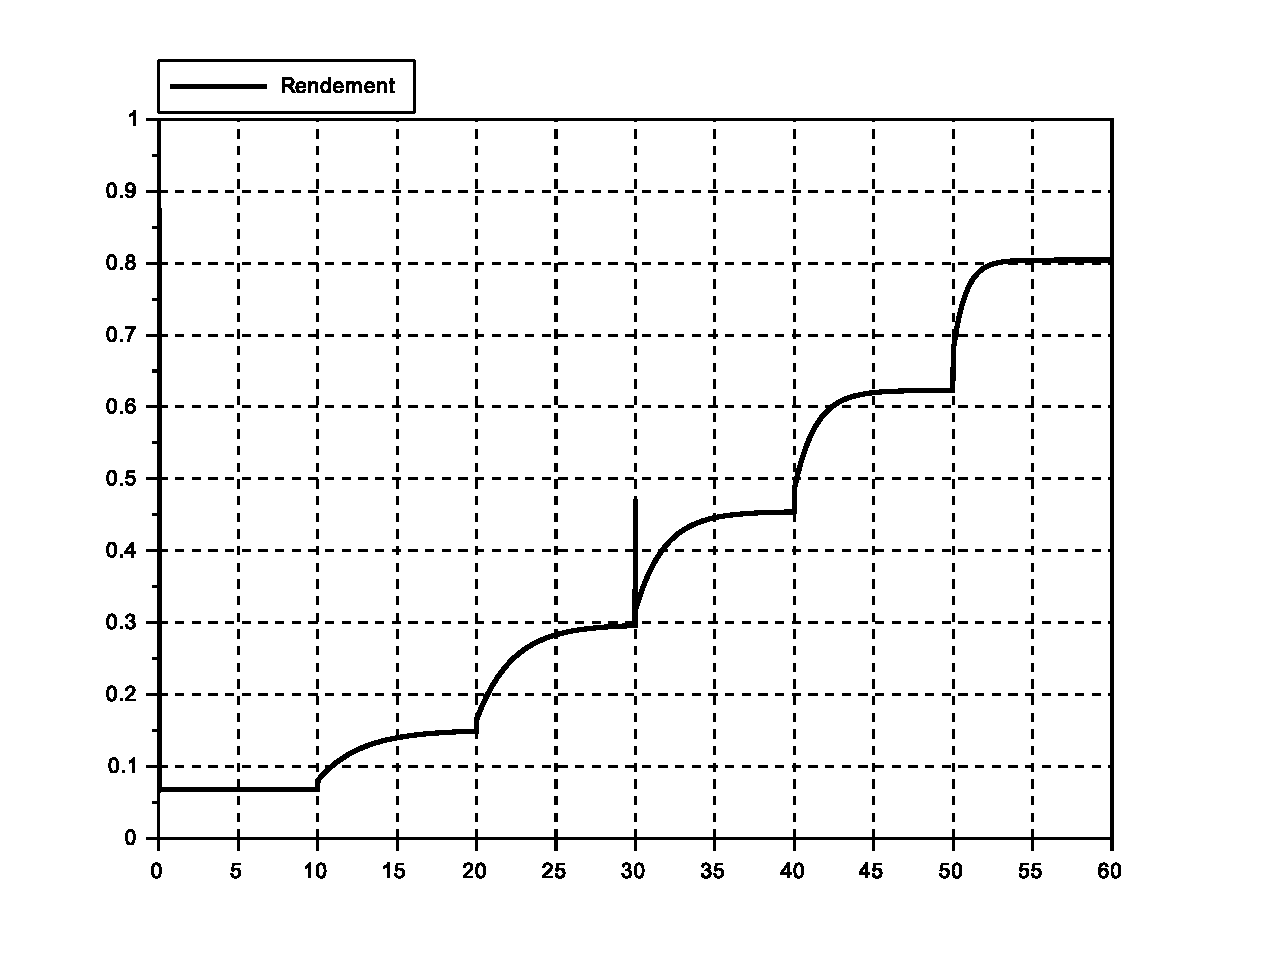
\includegraphics[width=0.8\linewidth]{img/Rendement}
\end{center}

\paragraph{Question 7:} Ce système a un rendement très faible lorsque la vitesse du moteur est faible. Il peut donc être utilisé afin de démarrer un moteur mais ne peut pas être utilisé comme un variateur classique. Nous verrons plus tard des solutions permettant d'améliorer les performances de ces systèmes.

\subsection{Flash d'appareil photo}

\paragraph{Question 1:}

$V_{in}(t)=u_{R_1}(t)+u_{R_2}(t)+u_C(t)$

$V_{in}(t)=(R_1+R_2).i(t)+u_C$

$V_{in}(t)=(R_1+R_2).C.\dfrac{du_C(t)}{dt}+u_C$

$V_{in}(p)=(R_1+R_2).C.p.U_C(p)+U_C(p)$

$\dfrac{U_C(p)}{V_{in}(p)}=\dfrac{1}{(R_1+R_2).C.p.+1}$

$\tau=(R_1+R_2).C=200.6*3.3*10^{-3}=0.66s$

$t_{5\%}=3\times 0.66=2s$

\paragraph{Question 2:}

$u_C(t)=V_{in}.\left(1-e^{-\dfrac{t}{(R_1+R_2).C}}\right)$

$u_C(t)=6.\left(1-e^{-\dfrac{t}{0.66}}\right)$

\paragraph{Question 3:}

$u_{R_3}(t)-u_C(t)=0$

$R_3*i(t)-u_C(t)=0$

$R_3*C.\dfrac{du_C(t)}{dt}+u_C(t)=0$

$R_3*C.(p.u_C(p)-u_C(0+))+u_C(p)=0$

$u_C(p)=u_C(0+).\dfrac{1}{R_3*C.p+1}$

$\tau=R_3*C=0.1*3.3*10^{-3}=0.33ms$

$t_{5\%}=1ms$

\paragraph{Question 4:}

$u_C(t)=V_{in}.e^{-\dfrac{t}{R_3.C}}$

$u_C(t)=6.e^{-\dfrac{t}{0.33*10^{-3}}}$

\paragraph{Question 5:}

\begin{center}
 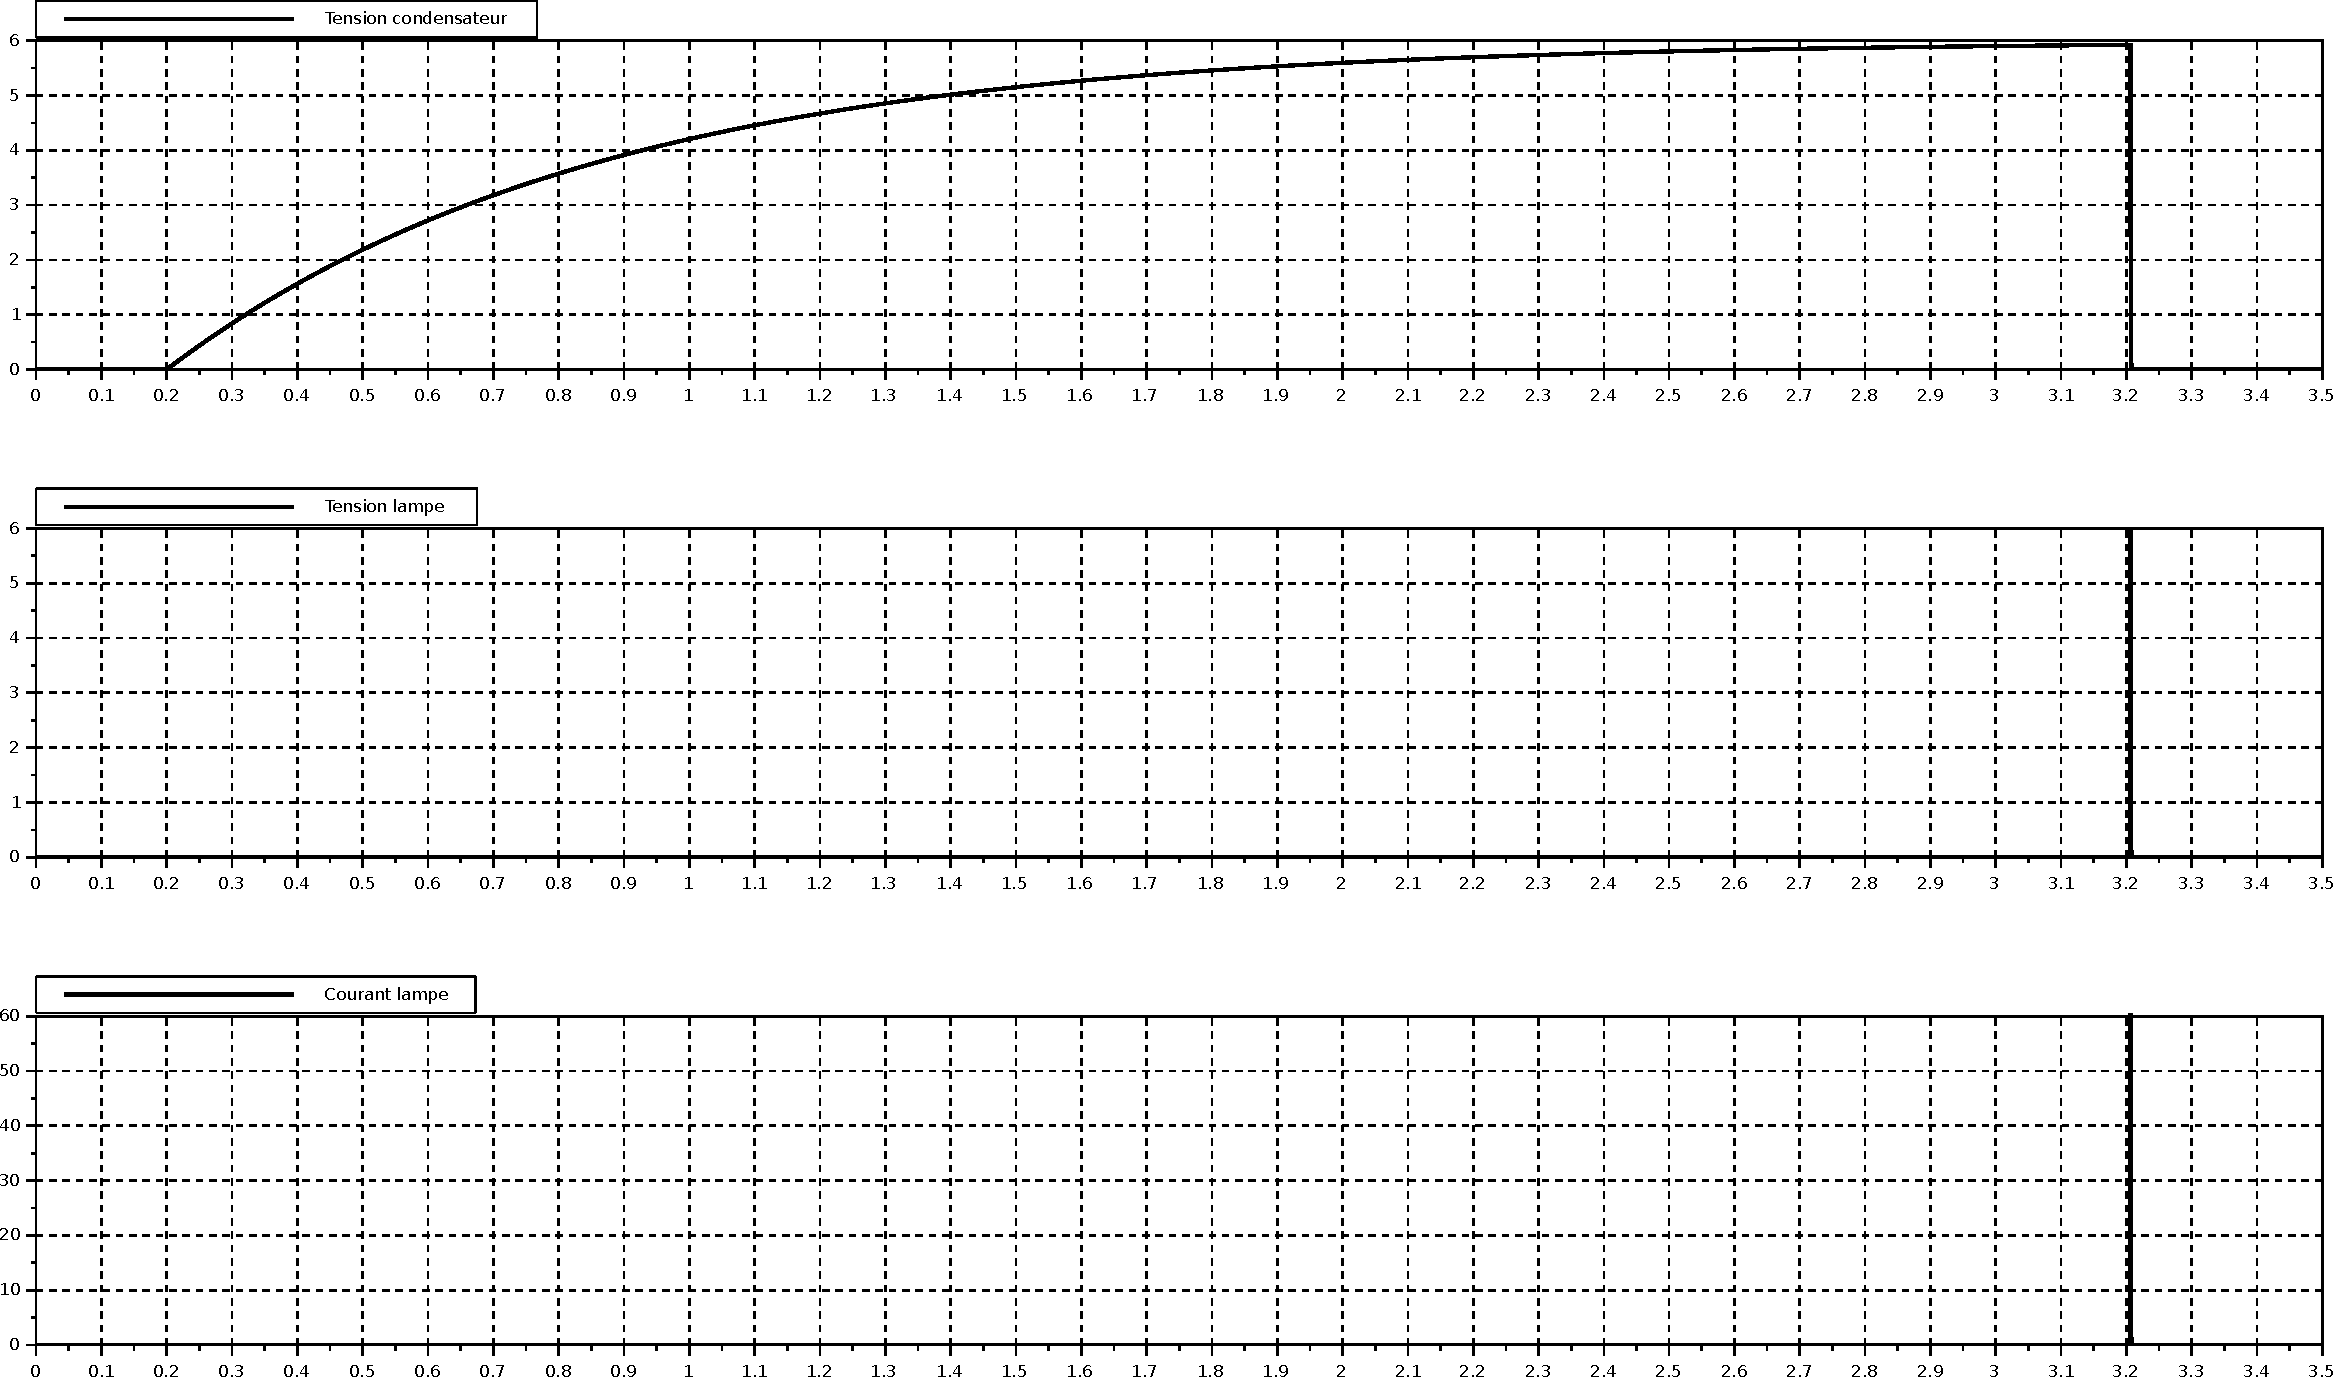
\includegraphics[width=0.8\linewidth]{img/Flash_results}
\end{center}

\subsection{Résistance de polarisation d'une DEL}

\paragraph{Question 1:} $i_R=i_F$

\paragraph{Question 2:} $U_R=V_{in}-V_F$

\paragraph{Question 3:} $U_R=R.i_R$

\paragraph{Question 4:} $V_{in}-V_F=R.i_F$

$i_F=\dfrac{V_{in}}{R}-\dfrac{V_F}{R}$

\paragraph{Question 5:} 

\begin{center}
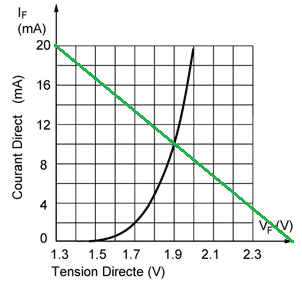
\includegraphics[width=0.5\linewidth]{img/DEL_carac_cor}
\end{center}

\paragraph{Question 6:} Graphiquement, on trouve $\dfrac{V_{in}-1.3}{R}=20mA$, donc $R=\dfrac{1.2}{20.10^{-3}}=60\Omega$.

\end{document}
